\documentclass[12pt,a4paper]{report}
\usepackage[utf8]{inputenc}
\usepackage[T1]{fontenc}
\usepackage{lmodern}
\usepackage{amsmath,amssymb}
\usepackage[margin=1in]{geometry}
\usepackage{setspace}
\usepackage{booktabs}
\usepackage{graphicx}
\usepackage{longtable}
\usepackage[hidelinks]{hyperref}
\usepackage{titlesec}
\titleformat{\chapter}[display]{\bfseries\Large}{\chaptertitlename\ \thechapter}{10pt}{\Large}
\onehalfspacing
\setlength{\parskip}{6pt}

\title{\bfseries Physical Interactions of Real-Time Drilling Parameters\\ and Their Application to
Latency Reduction in Drilling-Failure Alerting}
\author{Okeke Johnpaul Ebubechukwu\\ Matriculation No. 180808058\\[6pt]
Department of Petroleum and Gas Engineering\\ University of Lagos}
\date{\today}

\begin{document}
\maketitle
\tableofcontents
\listoffigures
\clearpage

\chapter{Introduction}

*Revised to the narrowed, physics-first scope: the interaction of real-time drilling parameters and its
exploitation to reduce failure-alert latency, with three machine-learning models as the applied
instrument rather than the subject.*

\section{Background to the Study}

Drilling a well is the most capital-intensive and least predictable phase of hydrocarbon development.
A significant fraction of rig time is consumed not by making hole but by \textbf{non-productive time (NPT)} ---
periods in which the drilling objective is suspended while a problem is diagnosed and remedied. Stuck
pipe, pack-off and poor hole cleaning, lost circulation, wellbore instability, premature bit failure and
well-control incidents account for the greater part of this lost time, and their cost is measured not only
in daily rig rate but in sidetracks, lost hole, fishing operations, and --- in the limiting case --- well
abandonment and personnel risk.

What makes these failures worth studying analytically is that most of them are \textbf{not instantaneous
events}. They are the terminal state of a physical process that develops over time. A cuttings bed does
not appear in an instant; it accumulates because the rate at which cuttings are generated at the bit
exceeds the rate at which the annular flow transports them away. A bit does not fail without warning; it
dulls progressively, and the energy required to remove a unit volume of rock rises as it does. A shale
does not always collapse abruptly; it can creep inward for hours when the mud weight sits below the
collapse pressure. In each of these cases the developing process perturbs the very quantities that are
already measured continuously at the rig floor and downhole --- weight on bit, torque, rate of penetration,
standpipe pressure, equivalent circulating density, hookload, flow rates, vibration.

This is the physical basis for \textbf{precursor-based monitoring}: if the process that produces a failure
evolves gradually, and if that evolution leaves a measurable trace in the acquired data, then the failure
can in principle be anticipated rather than merely recorded. Modern rigs generate exactly the data this
requires. Real-time surface and downhole measurements are logged at intervals of seconds, producing dense
multichannel time series over the life of a well. The Equinor \textbf{Volve} dataset --- the public release of a
complete field's subsurface and drilling data from the Norwegian Continental Shelf --- makes such data
available for open research, and has already been used to show that machine-learning methods can predict
well quantities from it as a time series (Olamigoke \& Onyeali, 2022).

A distinction of terms is useful here. \textbf{Predictive maintenance} infers the condition of equipment from
its operating signals so that intervention may be scheduled before failure; bit wear is its natural
drilling analogue, being a progressive deterioration in a component's condition, legible in the energy
required to do its work. The other mechanisms treated here --- pack-off, sticking, losses, instability --- are
more properly described as \textbf{failure prevention}, since what deteriorates is the wellbore rather than a
component. The diagnostic logic is common to both.

The difficulty is not data volume but \textbf{interpretation}. A single channel, read alone, is usually
ambiguous. Rising torque may indicate a developing pack-off, increased bit aggressiveness, a deviating
wellbore, or simply a change in formation. It acquires diagnostic meaning only in relation to the other
channels: torque interpreted together with weight on bit, rotary speed and rate of penetration is a
statement about drilling efficiency; interpreted together with standpipe pressure and equivalent
circulating density it is a statement about annular condition. The parameters are not independent
observations of separate phenomena --- they are \textbf{coupled responses of one hydraulic-mechanical system},
and a single physical cause typically perturbs several of them simultaneously and in a characteristic
pattern.

It is this structure --- which parameters are physically coupled, which carry independent information, and
what pattern each failure mechanism imprints across them --- that determines what can be detected, how
early, and how reliably. That structure is the subject of this study.

\section{Statement of the Problem}

Predictive systems for drilling failures are increasingly reported in the literature, and machine-learning
methods have been applied to stuck-pipe detection with encouraging results (Alshaikh et al., 2019; Mal et
al., 2022; Inoue et al., 2023; Al-Mamoori et al., 2025). Three limitations recur.

\textbf{First, the physics is frequently implicit.} Models are trained on raw channels or on generic
statistical features, with the physical mechanism of the failure left unexamined. Such a model may achieve
high accuracy on a particular dataset while offering no account of \emph{why} its inputs are informative --- and
consequently no basis for judging whether it will transfer to another well, another hole section, or
another rig. Where a model cannot explain the physical cause of its own alert, a drilling crew has little
reason to act on it.

\textbf{Second, the distinction between prediction and detection is often not drawn.} Failure modes differ
fundamentally in whether they admit early warning at all. Bit dulling develops over hours and can be
anticipated; a kick, by contrast, announces itself through flow and pit-volume changes *as the influx
begins*, not before. Reporting a single "prediction" capability across dissimilar modes conflates
mechanisms that provide genuine lead time with those for which only rapid detection is physically
possible, and thereby overstates what any system can deliver.

\textbf{Third, parameter interaction is rarely treated as the object of study, and the sensor suite is treated as
fixed.} Multivariate models exploit correlations between channels implicitly, in learned weights, without
establishing which correlations are physically meaningful, which channels are individually diagnostic, and
what the minimum set of measurements is that renders a given mechanism observable. Consequently such
systems are built around an assumed instrumentation set: the channels are taken as given, and the failures
addressed follow from that assumption. When a channel is unavailable --- a routine occurrence, since sensors
fail, rigs differ in equipment, and operators monitor different subsets --- the model either cannot run or
runs on degraded input without declaring that its diagnostic reach has narrowed. Neither behaviour is
acceptable in an operational setting, and both stem from the same omission: no explicit account of which
mechanisms a given set of parameters can and cannot observe.

The consequence is a gap between demonstrated statistical performance and defensible physical
understanding. \textbf{This study addresses that gap.} It treats the physical relationships among the monitored
drilling parameters as the primary object of investigation, establishes from those relationships what can
be predicted and on what timescale, and then applies machine-learning models as instruments to exploit
the relationships --- with the specific goal of quantifying how coupling between parameters, and
combination of complementary models, reduces the \textbf{latency} with which a developing failure is announced.

\section{Aim of the Study}

To investigate the physical relationships among real-time drilling parameters --- how they couple, how they
behave independently, and how those relationships can be exploited to reduce drilling-failure alert
latency --- and, on that basis, to develop a \textbf{composable monitoring framework} in which the failure
mechanisms a system can observe are \emph{derived from} the set of parameters it is given, instantiated using
three complementary machine-learning models (Random Forest, LSTM autoencoder, and Dynamic Time Warping)
fused into a single coverage-aware risk score.

The framing is deliberately two-layered. The \textbf{framework} establishes, from the physics, what any given
combination of monitored parameters can and cannot detect --- so that a monitoring configuration may be
assembled from one parameter, from three, or from a full sensor suite, with its diagnostic reach known in
advance rather than assumed. The \textbf{three-model ensemble} is the instrument through which that framework is
realised and tested.

\section{Specific Objectives}

1. To characterise, from first principles, the physical mechanisms of the principal drilling-failure modes
   --- bit wear, pack-off and poor hole cleaning, differential and mechanical sticking, lost circulation,
   wellbore instability, and kicks --- and the measurable signature each produces.
2. To quantify the interactions between the monitored parameters (equivalent circulating density,
   standpipe pressure, torque, rate of penetration, weight on bit, mechanical specific energy, and
   others), establishing which are physically coupled and which carry independent diagnostic information.
3. To derive and dimensionally verify the physical features that translate raw channels into
   mechanism-relevant quantities, including mechanical specific energy, the drilling exponent, equivalent
   circulating density, the cuttings-transport ratio, and the differential-sticking force.
4. To map each parameter to the failure mechanisms it can observe, distinguishing \emph{leading} (precursor)
   responses from \emph{coincident} ones, and thereby establishing what may be predicted as against only
   detected.
5. To determine, for each failure mechanism, the \textbf{minimum observable set} of parameters that renders it
   detectable --- and hence to establish a composable monitoring scheme in which an arbitrary selected
   subset of parameters yields a known, physically-derived set of observable mechanisms, together with an
   explicit statement of which mechanisms remain unobservable.
6. To apply three complementary machine-learning models --- Random Forest for point classification, an LSTM
   autoencoder for temporal anomaly detection, and Dynamic Time Warping for shape matching --- each
   targeting a distinct class of physical signature, and to fuse them into a single \textbf{coverage-aware} risk
   score whose weighting adjusts to the monitors actually available.
7. To determine the achievable lead time or detection latency for each failure mode from its physics, and
   to demonstrate how combining coupled parameters and the three models reduces alert latency relative to
   single-parameter, single-model monitoring.
8. To validate the parameter conventions, physical behaviours, and model outputs against the public
   Equinor Volve field data.

\section{Scope and Delimitation of the Study}

\textbf{Scope.} The study concerns the eight failure mechanisms named in Objective 1, analysed through
real-time surface and downhole drilling measurements. The empirical component uses the public Equinor
Volve dataset (block 15/9, licence PL 046, Norwegian Continental Shelf). Physical analysis proceeds from
established governing relations --- Teale's specific-energy formulation, the Jorden--Shirley drilling
exponent with the Rehm--McClendon correction, cuttings-transport relations after the Azar-group
experimental work, and the equivalent-circulating-density pressure balance.

\textbf{Delimitation.} Three boundaries are drawn deliberately.

\emph{On predictability.} The study does not claim uniform predictive capability across mechanisms. Prediction
with lead time is claimed only where the governing physics is dominated by gradual accumulation. Where a
mechanism builds a hazardous \emph{condition} whose moment of realisation is not signalled in advance --- notably
differential and mechanical sticking --- the output is an evolving \textbf{risk state}, not a timed forecast.
Where the physical signature coincides with the event itself, as for kicks, the objective is \textbf{minimised
detection latency} --- consistent with the well-control literature, in which the aim is early \emph{detection} of
an influx already under way rather than its prediction (Olamigoke \& James, 2022). This three-way
distinction is treated as a finding, not a limitation.

\emph{On implementation.} The system's software realisation --- alert delivery, user interface, deployment
architecture --- proceeds alongside this research but is \textbf{not} the subject of the report. The report
concerns the scientific and analytical basis: the parameter physics, the observability structure, and the
latency result.

\emph{On data.} Analysis is confined to channels present in the Volve release. Measurements that would
strengthen the treatment of wellbore instability in particular --- caliper logs and cavings observations ---
are not available, and conclusions on that mechanism are correspondingly qualified.

\section{Significance of the Study}

\textbf{To drilling practice.} Reduced alert latency has direct operational value: the earlier a developing
pack-off or a dulling bit is recognised, the wider the range of available remedies and the lower the
probability of escalation to stuck pipe or a lost hole section. By establishing the minimum set of
measurements that makes each mechanism observable, the study also offers guidance where instrumentation is
partial --- an ordinary rather than exceptional condition on working rigs.

\textbf{To the analytical literature.} The study contributes a physics-derived map between measured parameters
and failure mechanisms, with each relation classified by direction and by whether it \emph{leads} or merely
\emph{accompanies} the failure. This provides a basis for interpreting model behaviour physically rather than
statistically, and for stating honestly which mechanisms admit prediction.

\textbf{To monitoring-system design.} The principal methodological contribution is the treatment of
\textbf{diagnostic capability as a derived quantity rather than a fixed property}. Conventional monitoring
systems are built around a fixed sensor suite: the channels are assumed, and the failures addressed follow
from that assumption. Reversing the dependency, this study derives from the physics the minimum set of
parameters required to observe each mechanism, so that an arbitrary selected subset of parameters yields a
\emph{known} set of observable mechanisms --- and, equally important, an explicit statement of which mechanisms
that subset cannot see. A monitoring configuration may therefore be assembled around one parameter or
around a full suite, with its diagnostic reach established in advance and its blind spots declared rather
than concealed. Because the risk score renormalises over the monitors actually available, the system
degrades gracefully as instrumentation is reduced instead of failing silently or reporting a
falsely-confident result. This matters in practice because complete instrumentation is the exception on
working rigs, and it matters scientifically because a system that reports its own coverage is one whose
alerts can be trusted proportionately.

\textbf{To indigenous capability.} The work is conducted within a Nigerian university on a problem that costs
Nigerian operators directly through downtime and safety exposure, contributing to local competence in the
digital-oilfield methods increasingly central to the industry.

\section{Definition of Terms}

\textbf{Non-productive time (NPT).} Rig time during which the drilling objective is suspended while a problem
is addressed.

\textbf{Equivalent circulating density (ECD).} The effective density exerted at a depth during circulation,
comprising the static mud weight plus the equivalent contribution of annular friction pressure.

\textbf{Mechanical specific energy (MSE).} The mechanical energy expended per unit volume of rock removed,
combining axial and rotary work; an indicator of drilling efficiency and of bit condition (Teale, 1965).

\textbf{Precursor.} A measurable change in one or more channels that \emph{precedes} a failure and originates in the
physical process producing it --- as distinguished from a change that coincides with the failure.

\textbf{Lead time.} The interval between the earliest defensible alert and the failure event.

\textbf{Detection latency.} The interval between the physical onset of a failure and the moment it is announced;
the quantity minimised for mechanisms without precursors.

\textbf{Pack-off.} Restriction of the annulus by accumulated cuttings or cavings, raising circulating pressure
and drag, and a common precursor to stuck pipe.

\textbf{Differential sticking.} Immobilisation of the drill string against a permeable formation by the
pressure differential between wellbore and pore fluid acting over the contact area.

\textbf{Risk state.} A monitored condition indicating elevated likelihood of failure without a defensible
prediction of its timing.

\textbf{Minimum observable set.} The smallest group of channels whose simultaneous availability makes a given
mechanism detectable.

\section{Organisation of the Report}

\textbf{Chapter One} introduces the problem, aim, objectives and scope. \textbf{Chapter Two} reviews the physics of
the failure mechanisms and the literature on data-driven drilling-failure detection, establishing the
governing relations on which the analysis rests and positioning the study against existing work.
\textbf{Chapter Three} presents the methodology: derivation and dimensional verification of the physical
features, construction of the parameter--mechanism sensitivity map and the minimum observable sets, the
treatment of rig state and data conventions, and the formulation of the three models and their
coverage-aware fusion. \textbf{Chapter Four} presents and discusses the results --- the parameter-interaction
structure, the observable-mechanism sets obtained for selected parameter subsets, the per-mechanism latency
envelope, and the quantified reduction in alert latency. \textbf{Chapter Five} concludes and recommends further work.

\section*{References cited in this chapter}

Al-Mamoori, S.K., Tian, S. \& Ma, T. (2025) *Stuck Pipe Detection in Oil and Gas Drilling Operations Using
Deep Learning.* Applied Sciences. DOI: 10.3390/app15095042

Alshaikh, A., Magana-Mora, A., Gharbi, S. \& Al-Yami, A. (2019) *Machine Learning for Detecting Stuck Pipe
Incidents: Data Analytics.* IPTC. DOI: 10.2523/iptc-19394-ms

Inoue, K., Nakagawa, Y., Kaneko, T. \& Wada, R. (2023) *Early Stuck Pipe Detection Using Graph Attention
Machine Learning.* OMAE. DOI: 10.1115/omae2023-101928

Jorden, J.R. \& Shirley, O.J. (1966) \emph{Application of Drilling Performance Data to Overpressure Detection.}
JPT. DOI: 10.2118/1407-pa

Mal, S., Ødegård, S., Helgeland, S. \& Sinaga, Z. (2022) *Prediction of Stuck Pipe Incidents Using Models
Powered by Deep Learning.* SPE. DOI: 10.2118/208778-ms

Olamigoke, O. \& James, I. (2022) *Advances in Well Control: Early Kick Detection and Automated Control
Systems.* IntechOpen. DOI: 10.5772/intechopen.106800

Olamigoke, O. \& Onyeali, D.C. (2022) *Machine learning prediction of bottomhole flowing pressure as a time
series in the Volve field.* International Journal of Frontiers in Engineering and Technology Research, 2(2).
DOI: 10.53294/ijfetr.2022.2.2.0039

Rehm, B. \& McClendon, R. (1971) \emph{Measurement of Formation Pressure from Drilling Data.} SPE. DOI:
10.2118/3601-ms

Teale, R. (1965) \emph{The concept of specific energy in rock drilling.} International Journal of Rock
Mechanics and Mining Sciences. DOI: 10.1016/0148-9062(65)90022-7

Tomren, P.H., Iyoho, A.W. \& Azar, J.J. (1986) *Experimental Study of Cuttings Transport in Directional
Wells.* SPE Drilling Engineering. DOI: 10.2118/12123-pa

*Note on figures: Chapter One is deliberately figure-free; the timescale spectrum (`fig1`) and capability
graph (`fig7`) belong in Chapters Two and Three respectively, where they are derived.*


\chapter{Literature Review}

\section{Introduction}

This chapter establishes the two bodies of knowledge on which the study rests. The first is the \textbf{physics
of drilling failure}: the governing relations that determine how each mechanism develops and what it
imprints on the measured channels. The second is the \textbf{literature on data-driven failure detection},
against which the contribution of this work is positioned. The chapter is organised so that the physics
comes first and the models second, reflecting the study's premise that the physics determines what any
model can achieve.

§2.2 states the condition under which prediction is possible at all. §§2.3--2.9 treat each failure
mechanism. §2.10 draws out the parameter-interaction structure that follows from those mechanisms. §2.11
reviews data-driven detection methods, and §2.12 identifies the gap this study addresses.

\section{The condition for predictability: separation of timescales}

Whether a failure can be predicted is not a property of the algorithm applied to it but of the physical
process that produces it. A failure is predictable from measured data only if the process develops through
intermediate states that (i) leave a measurable signature in the available channels and (ii) evolve over a
time long compared with both the time needed to respond and the data sampling interval. Writing
$\tau_{\text{dev}}$ for the development time of the precursor, $\tau_{\text{resp}}$ for the response time,
and $\tau_{\text{sample}}$ for the sampling interval, prediction requires

\[\tau_{\text{dev}} \gg \tau_{\text{resp}} \gg \tau_{\text{sample}}\]

For real-time drilling data acquired at intervals of seconds, $\tau_{\text{sample}}$ is negligible; the
binding comparison is between $\tau_{\text{dev}}$ and $\tau_{\text{resp}}$. Where $\tau_{\text{dev}}$ is
tens of minutes to hours, an actionable warning is physically possible. Where $\tau_{\text{dev}}$
approaches $\tau_{\text{sample}}$, prediction degenerates into detection.

This condition is \textbf{necessary but not sufficient}. A slow process whose intermediate states leave no
distinguishable trace, or whose trace appears only simultaneously with the failure, provides no lead time
despite a long development. Both requirements --- a long development time \emph{and} a signature that leads the
event --- must hold. The mechanism-by-mechanism review that follows establishes which failures satisfy both.

\begin{figure}[htbp]\centering
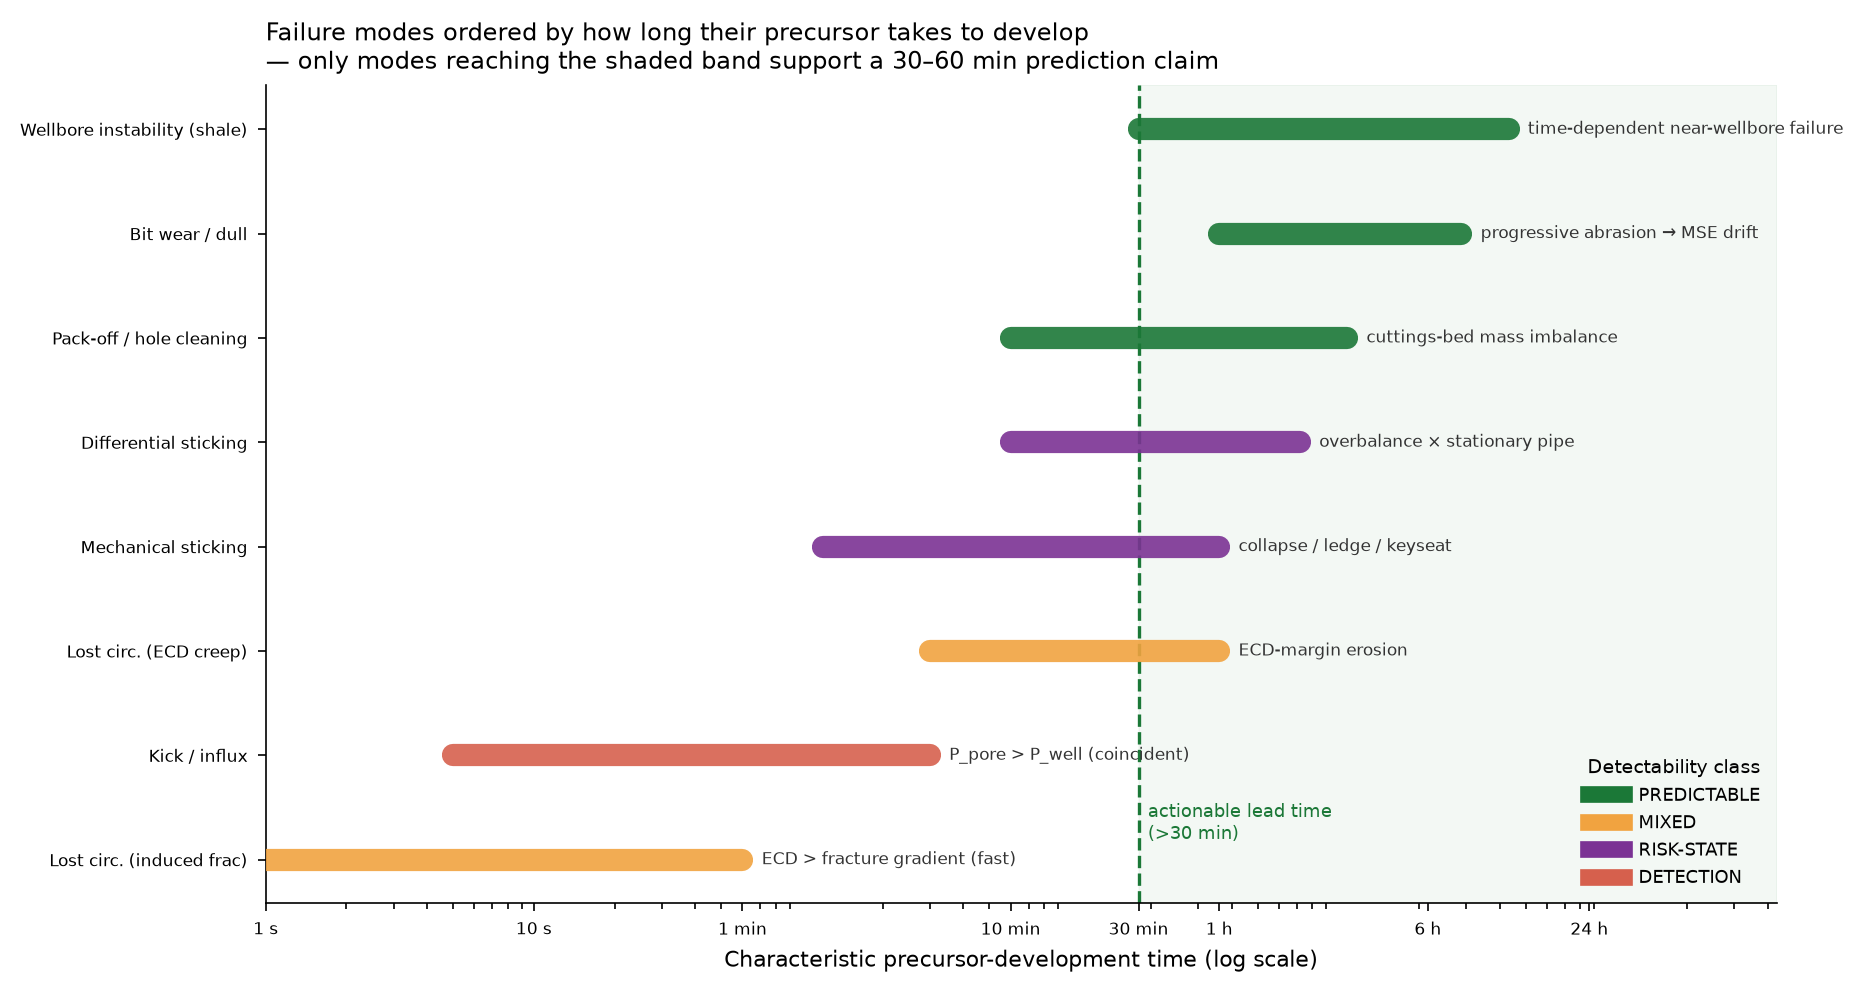
\includegraphics[width=\linewidth]{figures/fig1_timescale_spectrum.png}
\caption{Failure mechanisms ordered by the characteristic time over which their precursor develops (logarithmic axis). Only mechanisms extending into the shaded band admit an actionable warning of more than thirty minutes; colour denotes the detectability class established in this chapter.}\label{fig:2_1}
\end{figure}

\section{Hole cleaning and pack-off}

Pack-off is the restriction of the annulus by accumulated drilled cuttings or cavings. It is governed by a
mass balance between the rate at which cuttings enter the annulus at the bit and the rate at which the
annular flow removes them. Cuttings are generated at

\[Q_{\text{gen}} = \text{ROP} \cdot A_{\text{hole}}\]

and transported at

\[Q_{\text{trans}} = (v_{\text{ann}} - v_{\text{slip}}) \cdot A_{\text{ann}} \cdot C\]

where $v_{\text{ann}}$ is the annular fluid velocity, $v_{\text{slip}}$ the settling velocity of a
cutting relative to the fluid, $A_{\text{ann}}$ the annular flow area, and $C$ the transport efficiency.
The dimensionless \textbf{transport ratio} $R_t = Q_{\text{trans}} / Q_{\text{gen}}$ then determines the
outcome: for $R_t \geq 1$ cuttings are removed as fast as they are produced; for $R_t < 1$ a bed
accumulates at a rate proportional to the deficit.

The slip velocity follows, in the low-Reynolds-number limit, the Stokes relation

\[v_{\text{slip}} = \frac{g\,d_p^2\,(\rho_s - \rho_f)}{18\,\mu}\]

so that heavier cuttings, larger particles and thinner muds all reduce transport efficiency. Experimental
work on cuttings transport established the controlling variables and, importantly, the strong effect of
hole inclination: in the 30--60° range cuttings beds form readily and are difficult to remove, because the
gravitational component normal to the wellbore axis promotes settling while the axial flow does little to
re-entrain the settled material (Sifferman et al., 1974; Tomren, Iyoho \& Azar, 1986).

The consequences of an accumulating bed are the observable signature. A reduced annular flow area raises
frictional pressure loss, so \textbf{equivalent circulating density and standpipe pressure both rise};
mechanical interaction between the bed and the rotating string raises \textbf{torque and drag}. Because bed
growth is gradual --- accumulating over tens of minutes to hours --- pack-off satisfies both conditions of
§2.2 and is among the most predictable of drilling failures. It is also the mechanism whose signature is
most strongly \emph{multivariate}: a single physical cause perturbs several channels simultaneously and in a
characteristic correlated pattern, which is precisely the structure that multichannel monitoring can
exploit.

\begin{figure}[htbp]\centering
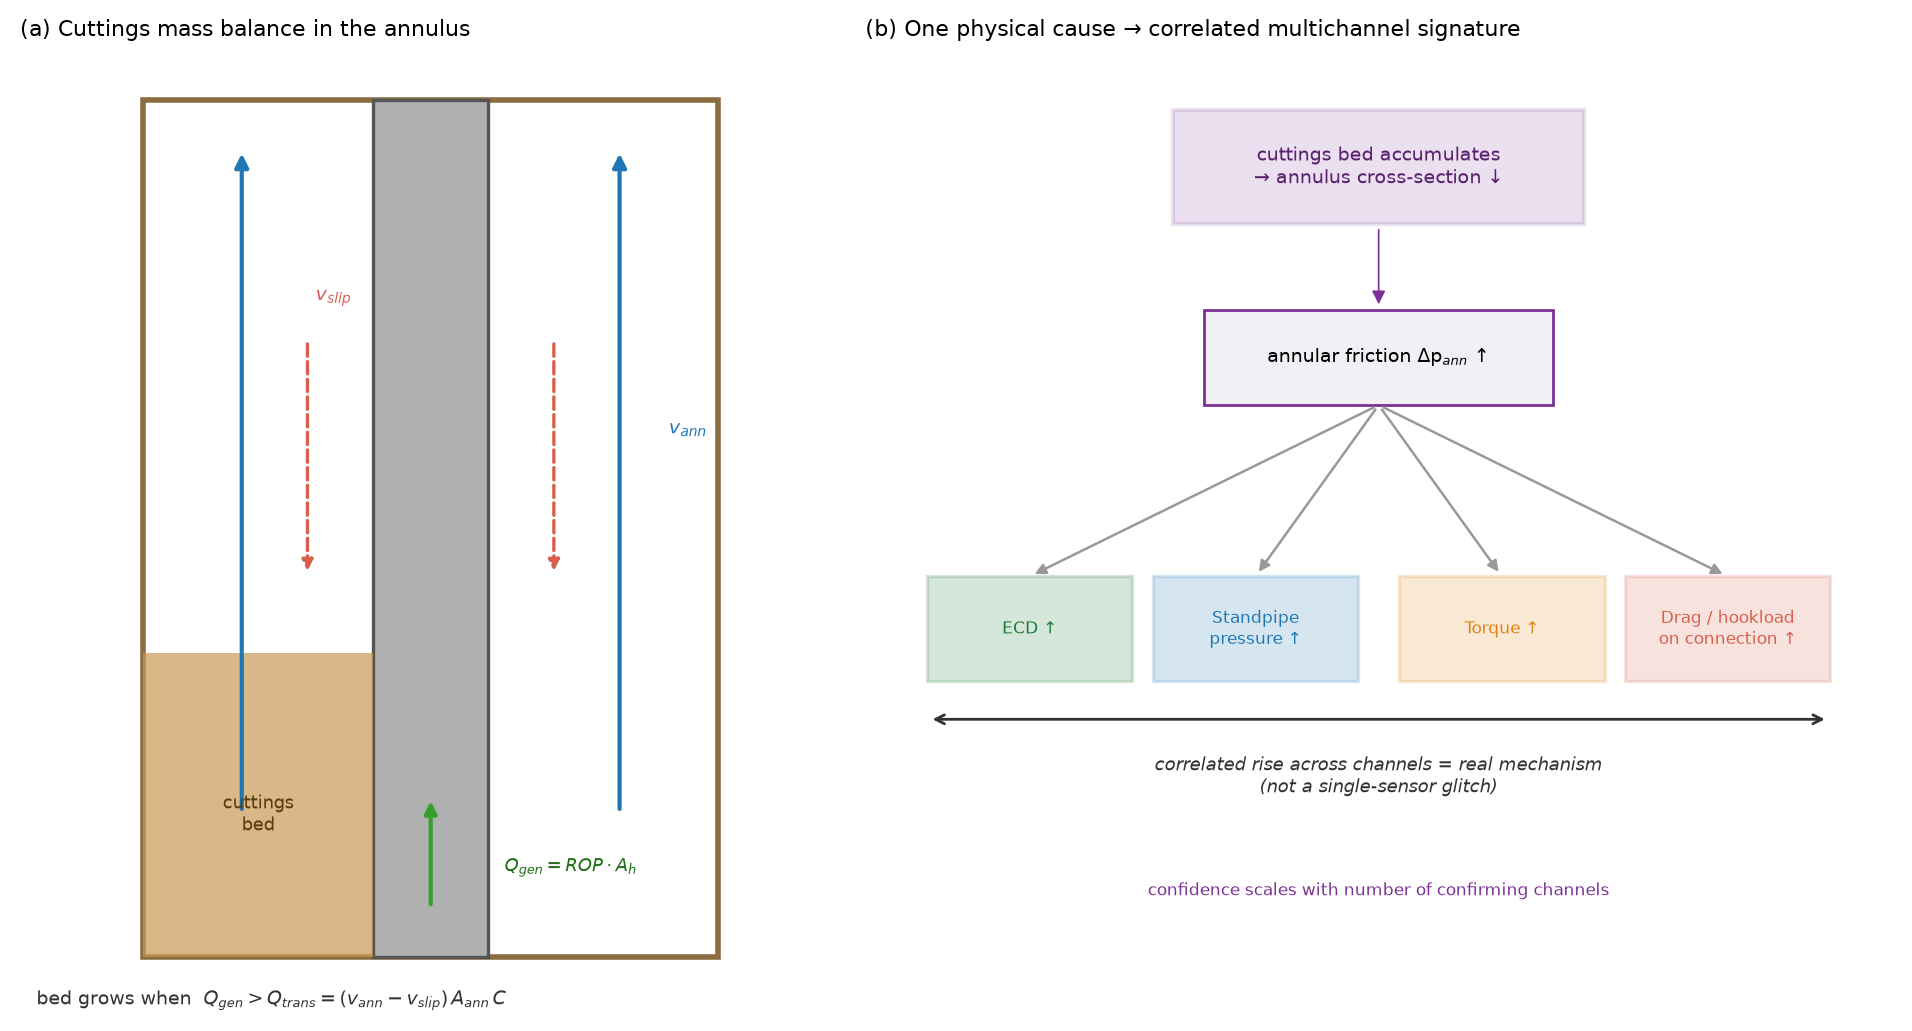
\includegraphics[width=\linewidth]{figures/fig2_packoff_mechanism.png}
\caption{Pack-off mechanism. (a) Cuttings mass balance in the annulus: a bed accumulates when the generation rate exceeds the transport rate. (b) The single physical cause propagates to several channels simultaneously, producing the correlated signature that distinguishes a real mechanism from a single-sensor fault.}\label{fig:2_2}
\end{figure}

\section{Bit wear and drilling efficiency}

The energy required to remove rock provides a direct measure of bit condition. Teale (1965) defined the
\textbf{mechanical specific energy} as the work done per unit volume of rock destroyed, comprising an axial and
a rotary contribution:

\[\text{MSE} = \frac{\text{WOB}}{A_b} + \frac{120\pi\,N\,T}{A_b \cdot \text{ROP}}\]

with WOB the weight on bit, $A_b$ the bit face area, $N$ the rotary speed, $T$ the torque and ROP the rate
of penetration. Teale further observed that in efficient drilling MSE approaches the compressive strength
of the rock; in practice, values of roughly 1.5--2 times the unconfined compressive strength indicate
efficient operation, while substantially higher values indicate energy being dissipated other than in
rock destruction.

As a bit dulls, more energy is required per unit volume removed: at fixed WOB and rotary speed, ROP falls
and torque rises, so \textbf{MSE increases progressively}. Dupriest \& Koederitz (2005) developed this into a
real-time surveillance method, using MSE trends to distinguish efficient drilling from \emph{founder} --- the
condition in which further increases in applied energy produce no additional penetration. Because bit
dulling proceeds over hours, it offers among the longest lead times of any mechanism considered here, and
its signature (rising MSE with falling ROP at constant input) is unambiguous provided formation change is
excluded as a confounder. That exclusion requires a formation-context channel such as gamma ray: an
increase in rock strength produces a similar MSE signature without any deterioration of the bit.

\begin{figure}[htbp]\centering
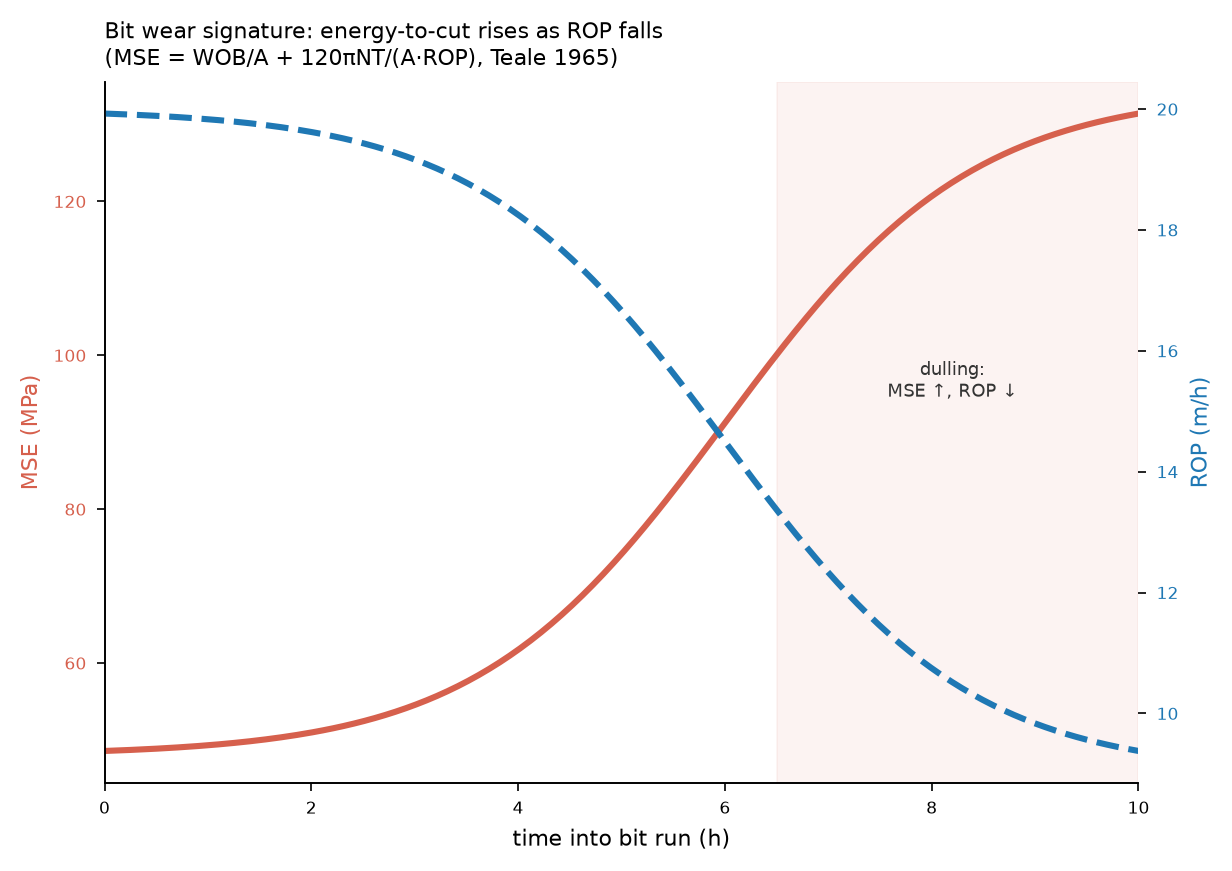
\includegraphics[width=\linewidth]{figures/fig4_mse_bitwear.png}
\caption{Bit-wear signature. As the bit dulls at constant weight on bit and rotary speed, the energy required per unit volume of rock removed rises while the rate of penetration falls. The crossover of the two trends is the diagnostic pattern.}\label{fig:2_3}
\end{figure}

\section{Pore pressure and the drilling exponent}

Drilling response also carries information about the formation being drilled. Jorden \& Shirley (1966)
introduced the \textbf{d-exponent}, a normalised measure of drillability:

\[d = \frac{\log_{10}\!\left(\dfrac{\text{ROP}}{60N}\right)}{\log_{10}\!\left(\dfrac{12\,\text{WOB}}{10^6 D}\right)}\]

with $D$ the bit diameter. Under normal compaction, increasing depth brings increasing rock strength and
the exponent rises steadily. Entry into an abnormally pressured formation reverses this: the pore fluid
supports part of the overburden, the rock is less compacted than its depth would suggest, drillability
improves, and the exponent departs downward from the established trend. Rehm \& McClendon (1971) corrected
the exponent for mud weight, giving

\[d_c = d \cdot \frac{\rho_{\text{normal}}}{\rho_{\text{actual}}}\]

which removes the confounding effect of mud-weight changes and makes the departure from trend
interpretable as a pore-pressure indicator.

\section{Well control and kick detection}

A kick begins when the pore pressure exceeds the wellbore pressure at some depth and formation fluid
enters the well:

\[P_{\text{pore}} > P_{\text{wellbore}} = 0.052 \cdot \text{ECD} \cdot \text{TVD}\]

The classical indicators --- flow out exceeding flow in, pit-volume gain, a drilling break, a standpipe
pressure fall, rising gas readings --- appear \textbf{as the influx begins}, not before it. The transition from
overbalance to underbalance may itself be gradual, but the observable signature is not: it coincides with
the event. Consequently kicks admit no precursor waveform leading the event by tens of minutes, and the
defensible objective is \textbf{minimising detection latency} rather than prediction. This is consistent with
the emphasis of the well-control literature on early \emph{detection} and automated response to an influx
already under way (Olamigoke \& James, 2022).

\section{Differential and mechanical sticking}

Differential sticking occurs when the drill string rests against a permeable formation and the pressure
differential between wellbore and pore fluid acts over the contact area:

\[F_{\text{stick}} = \Delta P \cdot A_{\text{contact}} \cdot f, \qquad \Delta P = P_{\text{wellbore}} - P_{\text{pore}}\]

The force grows with overbalance, with contact area --- itself increasing as filter cake builds and the
string embeds --- and with stationary time. This mechanism is physically distinct from those above in an
important respect. The overbalance and the contact geometry that make sticking likely are measurable and
evolve slowly, so the \textbf{risk} is observable; but the moment at which the string actually becomes
immobilised is not signalled in advance by any channel. The condition builds observably while its
realisation remains unpredictable in time.

The appropriate output for such a mechanism is therefore an evolving \textbf{risk state} rather than a timed
forecast. Mechanical sticking --- from keyseats, ledges, undergauge hole or collapsed formation --- shares
this character: the geometry that permits it can be inferred, but the event occurs when the string is
moved into the restriction.

\begin{figure}[htbp]\centering
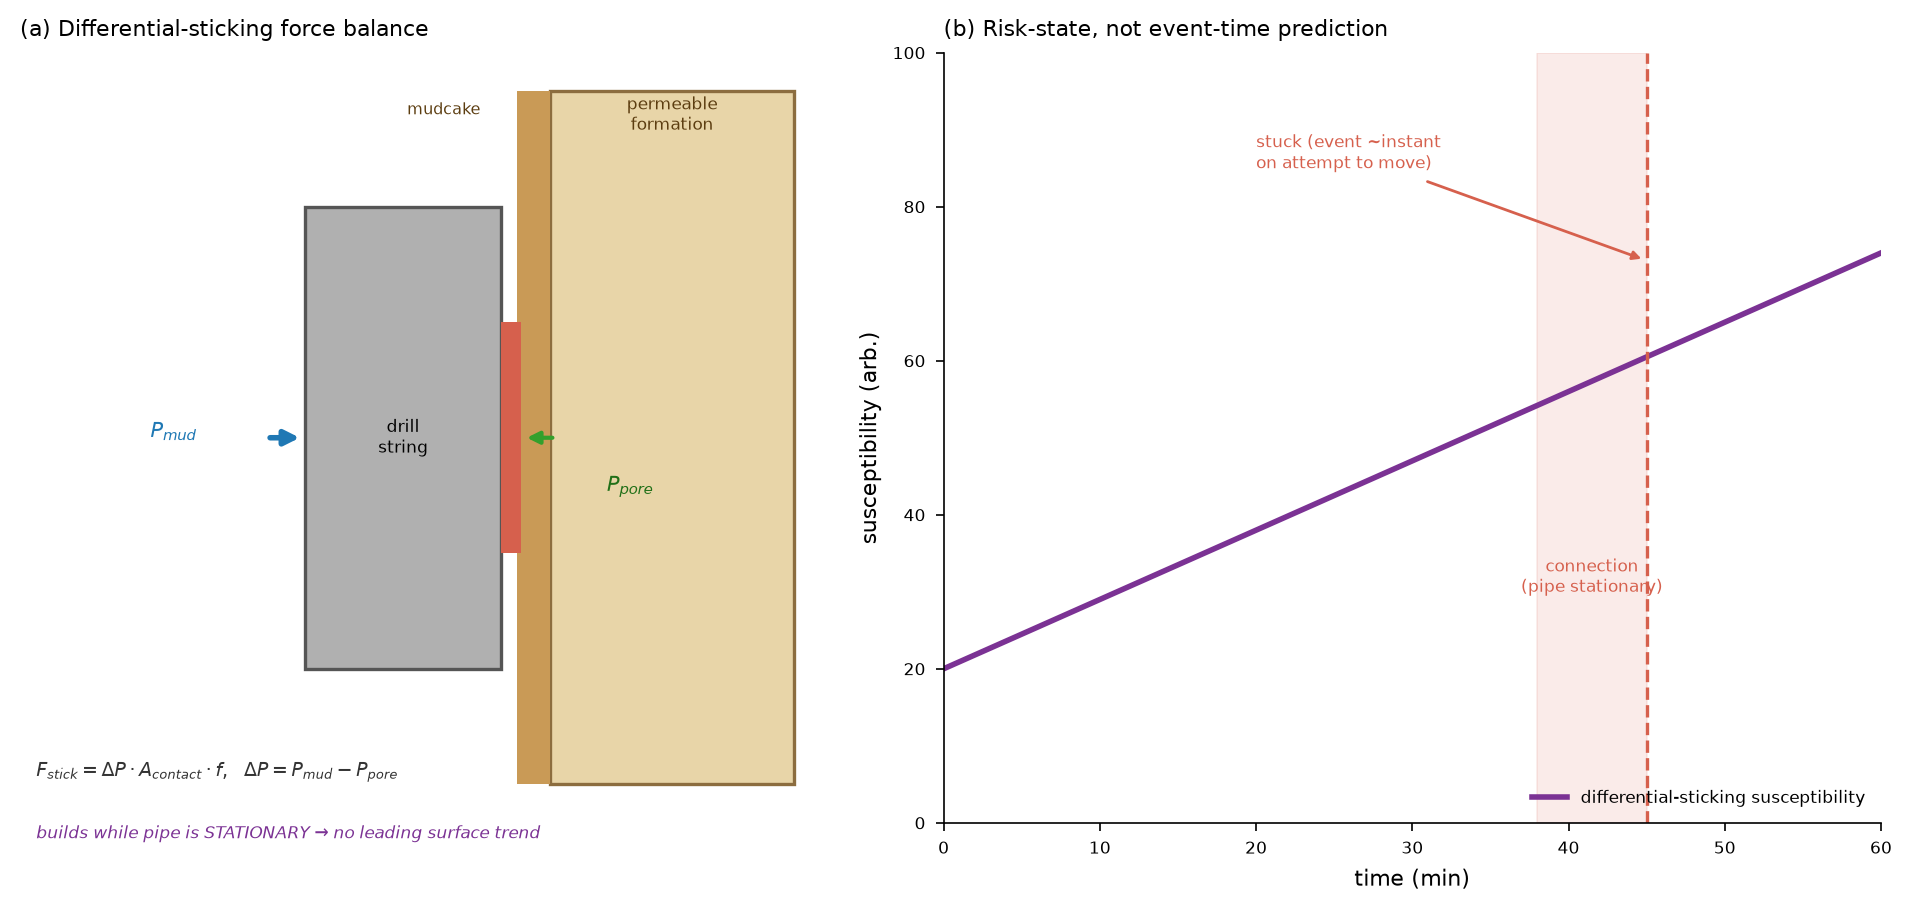
\includegraphics[width=\linewidth]{figures/fig3_diffstick_mechanism.png}
\caption{Differential sticking. (a) The force balance: overbalance acting across the contact area against a permeable formation. (b) Susceptibility grows observably while the pipe is stationary, but the event occurs on the attempt to move --- the basis for reporting a risk state rather than a timed prediction.}\label{fig:2_4}
\end{figure}

\section{Lost circulation}

Circulation is lost when the wellbore pressure exceeds the formation fracture gradient, or when the well
intersects an existing high-permeability path:

\[\text{ECD} > \text{FG}\]

where the equivalent circulating density combines the static mud weight with the annular friction
contribution,

\[\text{ECD} = \rho_{\text{mud}} + \frac{\Delta P_{\text{ann}}}{g \cdot \text{TVD}}\]

Two regimes follow, with different predictability. Where ECD creeps upward --- through cuttings loading,
increased flow rate, or narrowing annulus --- the approach to the fracture gradient is gradual and
observable in advance. Where the bit intersects a natural fracture or cavern, losses begin abruptly with
no leading signature. Lost circulation is therefore a \textbf{mixed} case, and reporting a single
predictability for it would misrepresent one regime or the other.

\section{Wellbore instability}

The stress concentration around a circular opening in a stressed medium is described by the Kirsch
solution; failure occurs where the induced stresses exceed the rock's strength envelope, commonly
represented by a Mohr--Coulomb criterion. Insufficient mud weight permits shear failure of the wall and
inward movement or breakout; excessive mud weight induces tensile failure. Between these lies the
operating window bounded below by the collapse pressure and above by the fracture gradient.

Shale instability has an additional time dependence: chemical interaction between mud and clay, and
pore-pressure diffusion into low-permeability rock, allow failure to develop over hours after a section is
drilled. The observable consequences are cavings production, an over-gauge hole, increased torque and
drag, and --- where cavings load the annulus --- the pack-off signature of §2.3. Mechanical earth models
constructed from log and offset data are used to establish the safe mud-weight window for a given
formation and stress state, and have been applied for wellbore-stability analysis in Niger Delta fields
(Adegbamigbe, Olamigoke \& Lawal, 2020). The mechanism is partially predictable: slow creep provides lead
time, brittle collapse may not, and the most direct confirming measurements --- caliper logs and cavings
observation --- are frequently unavailable in real-time data.

\section{The parameter-interaction structure implied by the physics}

Read together, §§2.3--2.9 establish a structural result that motivates this study. The monitored parameters
are not independent observations of separate phenomena: they are coupled responses of a single
hydraulic--mechanical system, and each failure mechanism perturbs a characteristic subset of them in a
characteristic pattern.

Three consequences follow.

\textbf{First, most channels are diagnostically ambiguous in isolation.} Rising torque is consistent with a
developing pack-off, with increased bit aggressiveness, with wellbore tortuosity, or with a change in
formation. It acquires meaning only in relation to other channels: with WOB, rotary speed and ROP it
describes drilling efficiency; with standpipe pressure and ECD it describes annular condition. A small
number of channels are exceptions --- torsional-vibration measurements such as a stick-slip index describe
a specific mechanism directly and are meaningful alone.

\textbf{Second, one physical cause produces several correlated responses.} A developing pack-off raises ECD,
standpipe pressure, torque and drag together. Agreement between channels that the physics predicts should
respond together is therefore evidence about the mechanism, not redundancy --- which is the basis for
treating multichannel confirmation as increased confidence.

\textbf{Third, rig state governs which physics applies.} Time-indexed drilling data contains long intervals in
which no hole is being made --- connections, tripping, circulating without rotation. During a connection the
rate of penetration falls to zero and depth ceases to advance, but this reflects the operation being
performed rather than any developing failure. Channels describing rig state --- block position, flow, hook
load, bit and hole depth --- therefore function as \emph{context}: they determine which mechanism physics is
valid at a given moment, and features such as MSE are undefined where ROP approaches zero.

\section{Data-driven detection of drilling failures}

Machine-learning approaches to drilling-failure detection have developed rapidly. Alshaikh et al. (2019)
applied data analytics to stuck-pipe incident detection using historical drilling records. Mal et al.
(2022) used deep-learning models for stuck-pipe prediction, and Inoue et al. (2023) applied a
graph-attention architecture to early stuck-pipe detection, using the learned attention structure to
represent relationships between channels. Al-Mamoori, Tian \& Ma (2025) report a deep-learning approach to
stuck-pipe detection in drilling operations. Work on the Volve dataset specifically has shown that
machine-learning methods can predict well quantities from it as time series (Olamigoke \& Onyeali, 2022).

Three method families recur, and they differ in the kind of departure they detect.

\textbf{Supervised classification} --- random forests, gradient boosting, support-vector methods --- learns a
decision boundary between labelled normal and abnormal operating points. It detects \emph{point} deviation:
whether the current multivariate state resembles states previously labelled as failures. Its dependence
on labels is also its limitation, since documented failure events are scarce.

\textbf{Unsupervised sequence models} --- most commonly autoencoders over recurrent or LSTM layers --- are trained
to reconstruct normal behaviour and score anomalies by reconstruction error (Nguyen, Tran \& Thomassey,
2020). They detect \emph{temporal} deviation: a trend departing from learned dynamics. They require no failure
labels, which suits a domain where labels are scarce, and they are well matched to precursors that are
gradual and correlated.

\textbf{Shape-based matching} --- chiefly dynamic time warping, with the Sakoe--Chiba band restricting the warping
path (Sakoe \& Chiba, 1978) --- compares a window against reference templates under elastic time alignment.
It detects \emph{shape} similarity: whether the recent trajectory resembles a known signature, irrespective of
its exact duration. It is well suited to mechanisms whose physics predicts a characteristic waveform.

That these three detect structurally different departures is the reason for combining them, and the
distinction is physical rather than statistical: point, trend and shape correspond to genuinely different
classes of signature in the drilling data.

\section{Gap in the literature}

Three limitations recur across the works reviewed.

\textbf{The physics is often implicit.} Models are trained on raw channels or generic statistical features,
without deriving why those inputs should be informative. A model achieving high accuracy on one dataset
thereby offers no account of its own transferability, and no physical explanation to justify acting on its
alerts.

\textbf{Prediction and detection are not consistently distinguished.} The mechanisms reviewed above differ
fundamentally: bit wear and pack-off develop observably over long periods; differential sticking builds an
observable risk whose timing is unsignalled; kicks announce themselves only as they begin. Reporting a
single predictive capability across these conflates categories and overstates what is achievable.

\textbf{The sensor set is treated as fixed.} Multivariate models exploit channel correlations implicitly, in
learned weights, without establishing which correlations are physically meaningful, which channels are
individually diagnostic, or what minimum set of measurements renders a mechanism observable. When a
channel is unavailable --- routine, since sensors fail and rigs differ in equipment --- such a model either
cannot run or runs on degraded input without declaring that its diagnostic reach has narrowed.

This study addresses these three gaps in order: it derives the mechanism physics first (§§2.3--2.9),
classifies mechanisms by what their physics permits, and derives from the mechanism--channel relationships
an explicit account of what a given set of parameters can and cannot observe. The three method families of
§2.11 are then applied as complementary instruments matched to the point, trend and shape signature
classes the physics identifies.

\section*{References}

Adegbamigbe, T., Olamigoke, O. \& Lawal, K.A. (2020) *Application of a 1-D Mechanical Earth Model for
Wellbore Stability Analysis in a Shallow-Water Field, Niger Delta.* SPE Nigeria Annual International
Conference and Exhibition. DOI: 10.2118/203632-ms

Al-Mamoori, S.K., Tian, S. \& Ma, T. (2025) *Stuck Pipe Detection in Oil and Gas Drilling Operations Using
Deep Learning.* Applied Sciences. DOI: 10.3390/app15095042

Alshaikh, A., Magana-Mora, A., Gharbi, S. \& Al-Yami, A. (2019) *Machine Learning for Detecting Stuck Pipe
Incidents: Data Analytics.* IPTC. DOI: 10.2523/iptc-19394-ms

Dupriest, F.E. \& Koederitz, W.L. (2005) *Maximizing Drill Rates with Real-Time Surveillance of Mechanical
Specific Energy.* SPE/IADC Drilling Conference. DOI: 10.2523/92194-ms

Inoue, K., Nakagawa, Y., Kaneko, T. \& Wada, R. (2023) *Early Stuck Pipe Detection Using Graph Attention
Machine Learning.* OMAE. DOI: 10.1115/omae2023-101928

Jorden, J.R. \& Shirley, O.J. (1966) \emph{Application of Drilling Performance Data to Overpressure Detection.}
Journal of Petroleum Technology. DOI: 10.2118/1407-pa

Mal, S., Ødegård, S., Helgeland, S. \& Sinaga, Z. (2022) *Prediction of Stuck Pipe Incidents Using Models
Powered by Deep Learning.* SPE. DOI: 10.2118/208778-ms

Nguyen, H.D., Tran, K.P. \& Thomassey, S. (2020) *Forecasting and Anomaly Detection approaches using LSTM
and LSTM Autoencoder techniques.* International Journal of Information Management. DOI:
10.1016/j.ijinfomgt.2020.102282

Olamigoke, O. \& James, I. (2022) *Advances in Well Control: Early Kick Detection and Automated Control
Systems.* IntechOpen. DOI: 10.5772/intechopen.106800

Olamigoke, O. \& Onyeali, D.C. (2022) *Machine learning prediction of bottomhole flowing pressure as a time
series in the Volve field.* International Journal of Frontiers in Engineering and Technology Research,
2(2). DOI: 10.53294/ijfetr.2022.2.2.0039

Rehm, B. \& McClendon, R. (1971) \emph{Measurement of Formation Pressure from Drilling Data.} SPE. DOI:
10.2118/3601-ms

Sakoe, H. \& Chiba, S. (1978) \emph{Dynamic programming algorithm optimization for spoken word recognition.}
IEEE Transactions on Acoustics, Speech and Signal Processing. DOI: 10.1109/tassp.1978.1163055

Sifferman, T.R., Myers, G.M. \& Haden, E.L. (1974) \emph{Drill Cutting Transport in Full Scale Vertical Annuli.}
Journal of Petroleum Technology. DOI: 10.2118/4514-pa

Teale, R. (1965) \emph{The concept of specific energy in rock drilling.} International Journal of Rock
Mechanics and Mining Sciences. DOI: 10.1016/0148-9062(65)90022-7

Tomren, P.H., Iyoho, A.W. \& Azar, J.J. (1986) *Experimental Study of Cuttings Transport in Directional
Wells.* SPE Drilling Engineering. DOI: 10.2118/12123-pa


\chapter{Methodology}

\section{Introduction and research design}

The study proceeds in a deliberate order: the physics is established and verified first, and only then are
models applied. This ordering is methodological rather than presentational. Because the physics determines
which mechanisms admit prediction, what each feature measures, and which channels can observe which
mechanism, establishing it first means every subsequent modelling choice can be justified physically ---
and any model output that contradicts the physics can be recognised as an error rather than a discovery.

Five stages follow. §3.2 derives the physical features and verifies them dimensionally. §3.3 constructs the
parameter--mechanism sensitivity map and the minimum observable sets. §3.4 establishes the data conventions
and rig-state gating rules. §3.5 formulates the three models and their coverage-aware fusion. §3.6 defines
the evaluation, including the ablation design that produces the latency result.

\section{Derivation and dimensional verification of physical features}

Twelve features translate raw measured channels into mechanism-relevant physical quantities. Each is
implemented in both \textbf{field} and \textbf{SI} forms, since the governing relations appear in the literature in
field units while the Volve dataset is metric.

\begin{center}\small
\begin{tabular}{llll}
\toprule
# & Feature & Physical meaning & Mechanism informed \\
\midrule
1 & Mechanical specific energy & energy per unit rock volume removed & bit wear, founder \\
2 & d-exponent & normalised drillability & pore pressure \\
3 & Corrected exponent $d_c$ & drillability, mud-weight corrected & overpressure \\
4 & Equivalent circulating density & dynamic pressure as density & pressure window \\
5 & ECD margin & distance to fracture gradient & losses, instability \\
6 & Transport ratio & cuttings removed / cuttings generated & hole cleaning \\
7 & Slip velocity & cutting settling velocity & hole cleaning \\
8 & Annular velocity & mean annular fluid velocity & hole cleaning \\
9 & Overbalance & wellbore minus pore pressure & differential sticking \\
10 & Sticking force & overbalance force on contact area & differential sticking \\
11 & Stick-slip index & torsional-vibration severity & stick-slip \\
12 & Hydraulic horsepower & power delivered at the bit & bit hydraulics \\
\bottomrule
\end{tabular}\end{center}

\textbf{Dimensional verification.} Each relation is checked symbolically by reducing both sides to the base
dimensions of mass, length and time and asserting equality. This is implemented with a computer-algebra
system and executed as a self-test whenever the feature module is loaded, so a unit error cannot enter the
pipeline silently. All checks pass. Representative results:

\begin{center}\small
\begin{tabular}{lll}
\toprule
Relation & Reduces to & Expected \\
\midrule
Cuttings generation and transport rates & $L^3 T^{-1}$ & volumetric flow ✓ \\
Transport ratio & dimensionless & ✓ \\
Slip velocity & $L T^{-1}$ & velocity ✓ \\
ECD annular term & $M L^{-3}$ & density ✓ \\
Sticking force & $M L T^{-2}$ & force ✓ \\
MSE, both terms & $M L^{-1} T^{-2}$ & pressure ✓ \\
\bottomrule
\end{tabular}\end{center}

\textbf{Numerical cross-validation.} Beyond dimensional consistency, the field and SI implementations are
evaluated on the same physical state and required to agree. For mechanical specific energy the two forms
agree to within 0.4 \%, confirming the unit conversions. A representative efficient-drilling state returns
MSE ≈ 1.7 times the unconfined compressive strength of the rock, within the 1.5--2 range Teale's
formulation predicts for efficient operation --- an independent check that the implementation reproduces
known physical behaviour.

\begin{figure}[htbp]\centering
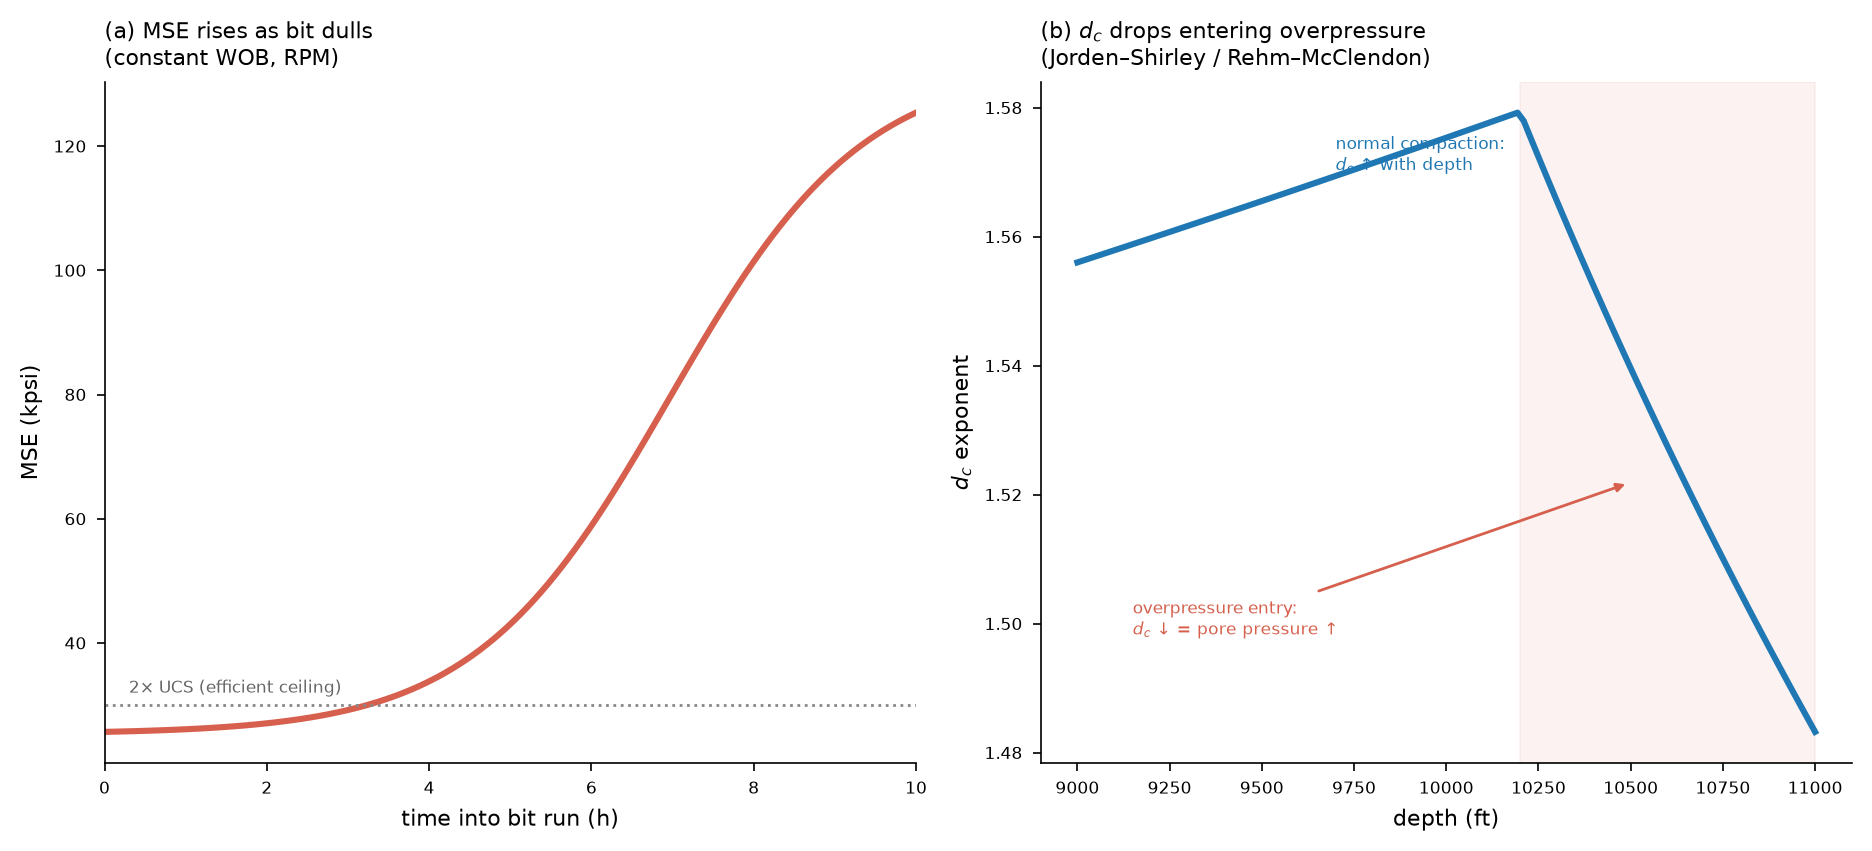
\includegraphics[width=\linewidth]{figures/fig5_feature_worked_example.png}
\caption{Worked example of two derived features. (a) Mechanical specific energy rising past the efficient-drilling ceiling as the bit dulls. (b) The corrected exponent rising with depth under normal compaction, then departing downward on entry to an overpressured formation.}\label{fig:3_1}
\end{figure}

\textbf{Corrections to published forms.} Three errors in the formulations initially adopted for this work were
identified and corrected during verification: downhole pressure had been expressed in pounds per gallon, a
density unit, and is correctly expressed in pressure units, with pounds per gallon reserved for mud weight
and ECD; the d-exponent expression contained transcription errors in both numerator and denominator; and
the MSE expression did not reduce to Teale's form. Each was corrected against the primary source and
re-verified.

\section{The parameter--mechanism sensitivity map}

The physics of Chapter Two predicts, for each mechanism, which channels respond, in which direction, and
whether the response \emph{leads} the failure or merely accompanies it. These predictions are assembled into a
sensitivity matrix over sixteen channels and eight mechanisms.

\textbf{Encoding.} Each cell records the direction of response --- increase, decrease, or either --- together with
its temporal role: \textbf{leading} (the channel moves before the event, so prediction is possible),
\textbf{coincident} (the channel moves as the event occurs, supporting detection only), or \textbf{context} (the
channel does not indicate the mechanism but conditions whether its physics applies).

\textbf{Channel clusters.} The sixteen channels group into four physical clusters, which is why the matrix is
structured rather than arbitrary: \emph{mechanical} (weight on bit, rotary speed, torque, rate of penetration,
stick-slip, shock), \emph{hydraulic} (standpipe pressure, ECD, downhole pressure, flow, mud weight, pit
volume), \emph{formation} (gamma ray, downhole temperature), and \emph{rig state} (block position, hook load). Each
mechanism draws principally on one cluster, with rig-state channels acting across all as gates.

\begin{figure}[htbp]\centering
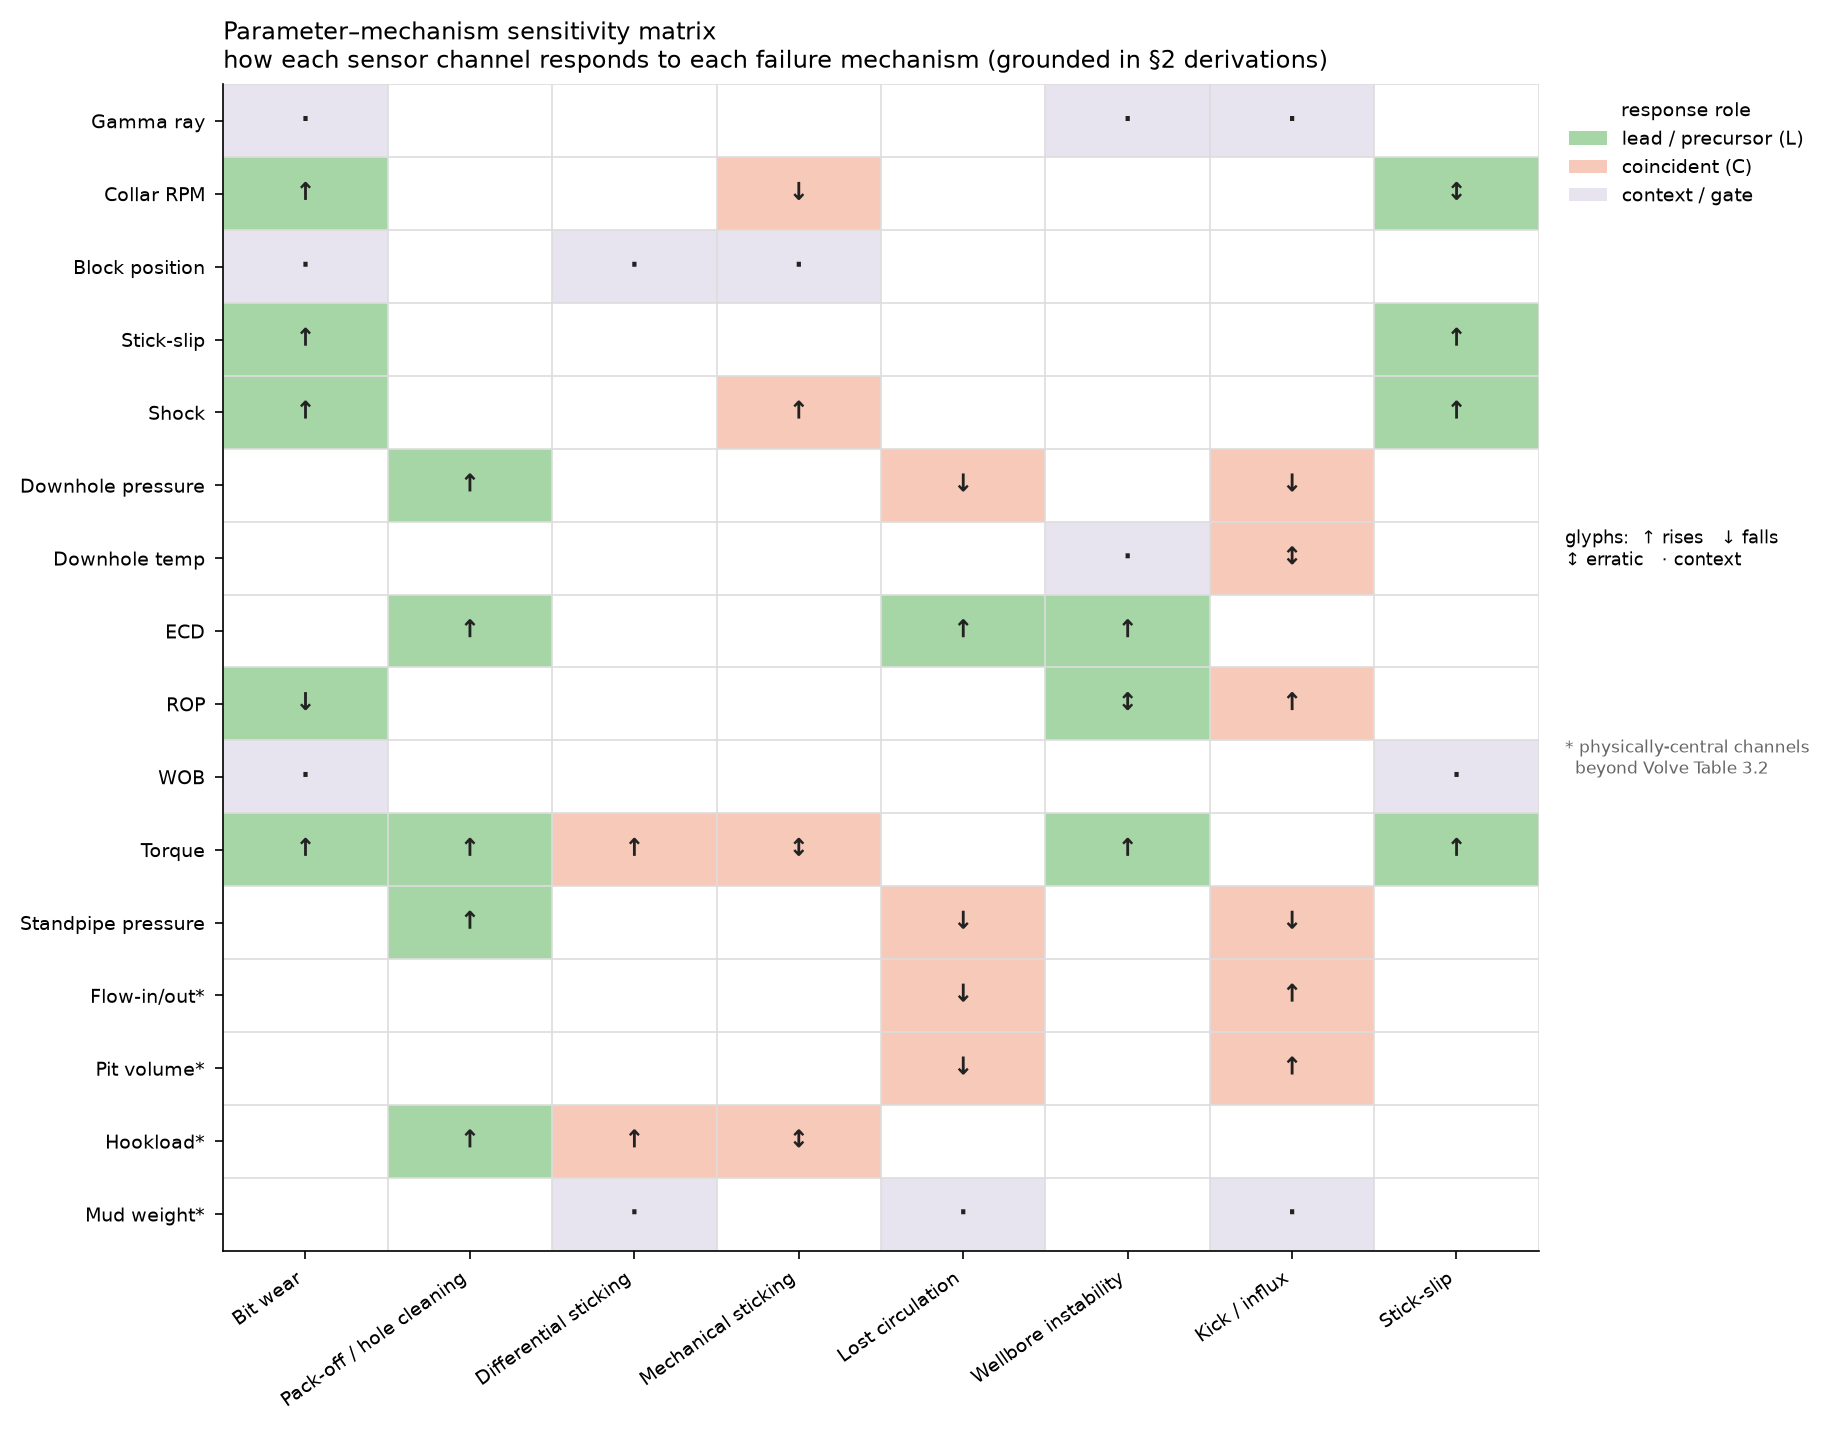
\includegraphics[width=\linewidth]{figures/fig6_sensitivity_matrix.png}
\caption{The parameter--mechanism sensitivity matrix. Each cell records the direction of a channel's response to a mechanism and its temporal role: leading, coincident, or context. Empty cells denote no physically-expected response.}\label{fig:3_2}
\end{figure}

\textbf{Minimum observable sets.} From the matrix, the smallest set of channels that makes each mechanism
detectable is derived. These sets are the formal basis of the composable framework: given any selected
subset of channels, the observable mechanisms are exactly those whose minimum observable set is contained
in the selection, and the remainder are explicitly unobservable.

\begin{center}\small
\begin{tabular}{lll}
\toprule
Mechanism & Minimum observable set & Size \\
\midrule
Stick-slip & stick-slip index alone & 1 \\
Kick / influx & flow in/out, pit volume & 2 \\
Pack-off & ECD, standpipe pressure, torque & 3 \\
Differential sticking & overbalance, hook load, rig state & 3 \\
Mechanical sticking & torque, hook load, rig state & 3 \\
Lost circulation & flow in/out, pit volume, ECD & 3 \\
Wellbore instability & torque, drag, ECD \emph{(partial --- caliper and cavings unavailable)} & 3 \\
Bit wear & weight on bit, rotary speed, torque, rate of penetration & 4 \\
\bottomrule
\end{tabular}\end{center}

Two results from this construction bear on the study's claims. First, \textbf{stick-slip is the only mechanism
observable from a single channel} --- the torsional-vibration measurement is self-diagnostic, whereas
torque, standpipe pressure and ECD are relational and near-uninformative alone. Second, the mechanisms
classified in Chapter Two as risk-state or detection-only carry \textbf{zero leading channels}, which
independently confirms that classification from the matrix rather than by assertion.

\begin{figure}[htbp]\centering
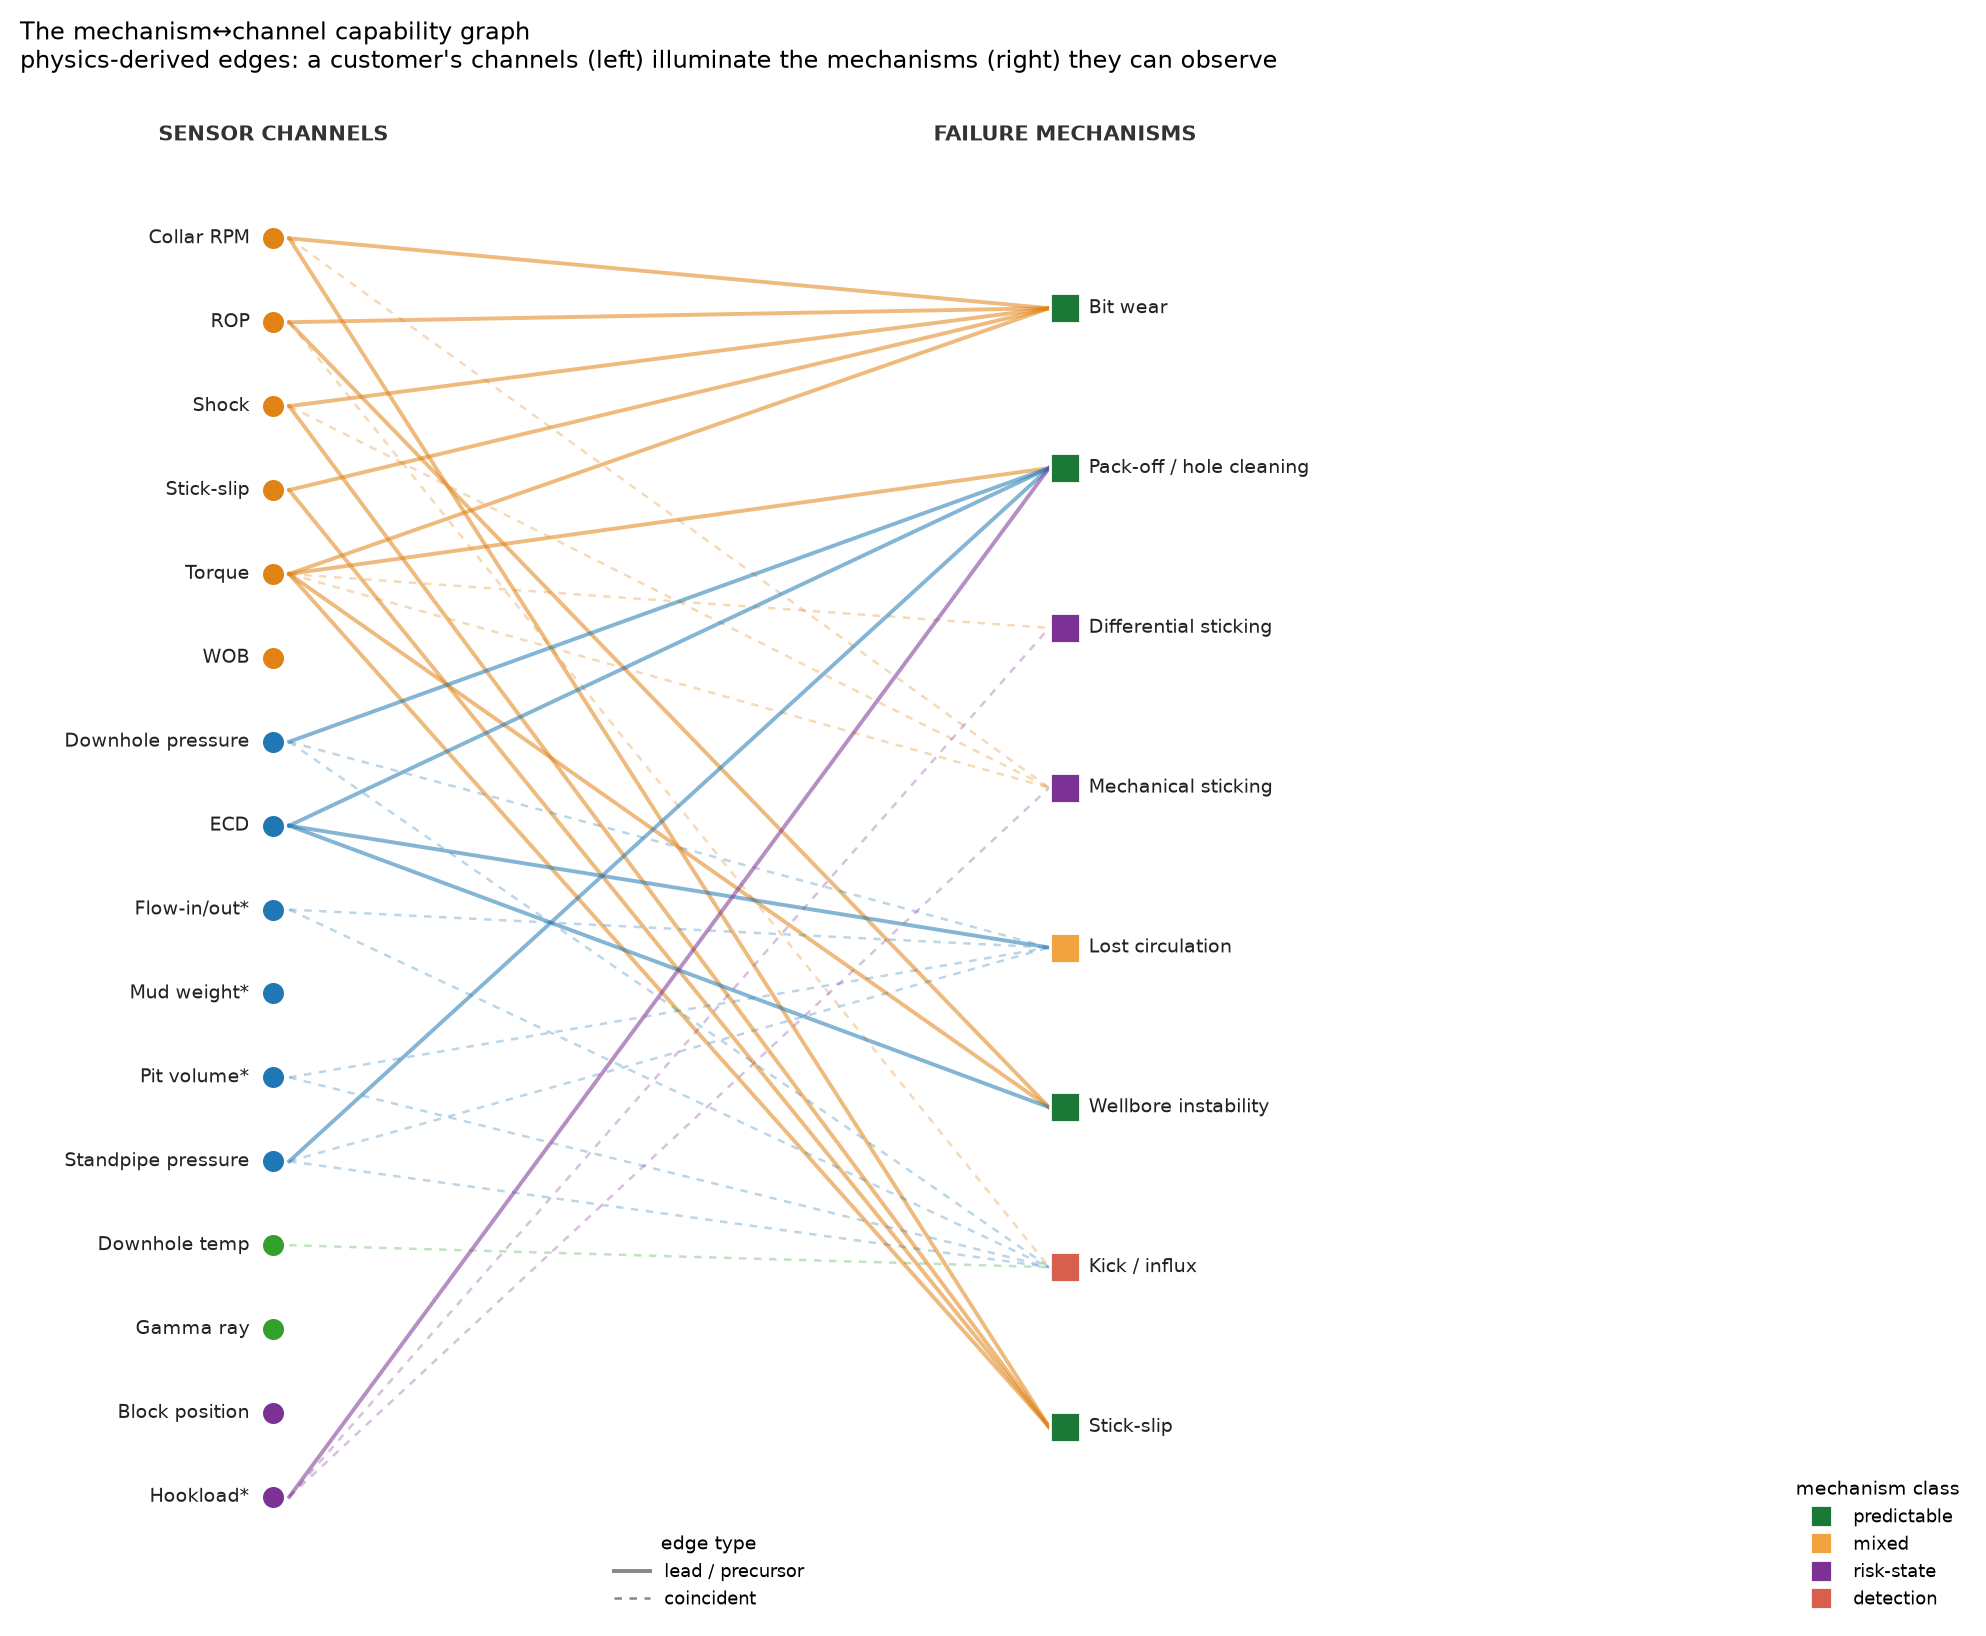
\includegraphics[width=\linewidth]{figures/fig7_capability_graph.png}
\caption{The mechanism--channel capability graph. Sensor channels (left, grouped by physical cluster) connect to failure mechanisms (right, coloured by detectability class) through physics-derived edges; solid edges denote a leading response, dashed a coincident one. The mechanisms a given channel selection can observe are those whose required edges it covers.}\label{fig:3_3}
\end{figure}

\section{Data source, conventions and rig-state gating}

\textbf{Dataset.} The study uses the public Equinor Volve dataset from block 15/9 (licence PL 046) on the
Norwegian Continental Shelf, comprising well logs, drilling records and real-time surface measurements for
wells of the 15/9-F series. Real-time drilling data are time-indexed at intervals of seconds. The specific
wellbore analysed is identified from the file headers rather than assumed.

\textbf{Unit conventions.} Volve is a metric dataset: depths in metres, penetration rate in metres per hour,
pressures in bar or kilopascals, mud weight in specific gravity or kilograms per cubic metre. The SI
feature forms of §3.2 are therefore the primary implementation, with the field forms retained for
cross-checking. Each channel's unit is read from its header rather than inferred.

\textbf{Rig-state gating.} Because the data is time-indexed rather than depth-indexed, it contains extended
intervals in which no hole is being made. At every pipe connection the rate of penetration falls to zero
and bit depth ceases to advance --- a consequence of the operation being performed, not of any developing
failure. Two errors follow if this is ignored: an ungated model raises an alarm at every connection, and
MSE diverges as ROP approaches zero.

A boolean mask is therefore constructed from the rig-state channels, requiring circulation (flow above
threshold), the bit on bottom (hole depth minus bit depth within tolerance) and hole being made. Mechanism
features are computed only where this mask holds, and the fraction of samples retained is reported as a
data-quality measure. This is the operational meaning of treating rig-state channels as context: they
determine which physics is valid before any feature is evaluated.

\begin{figure}[htbp]\centering
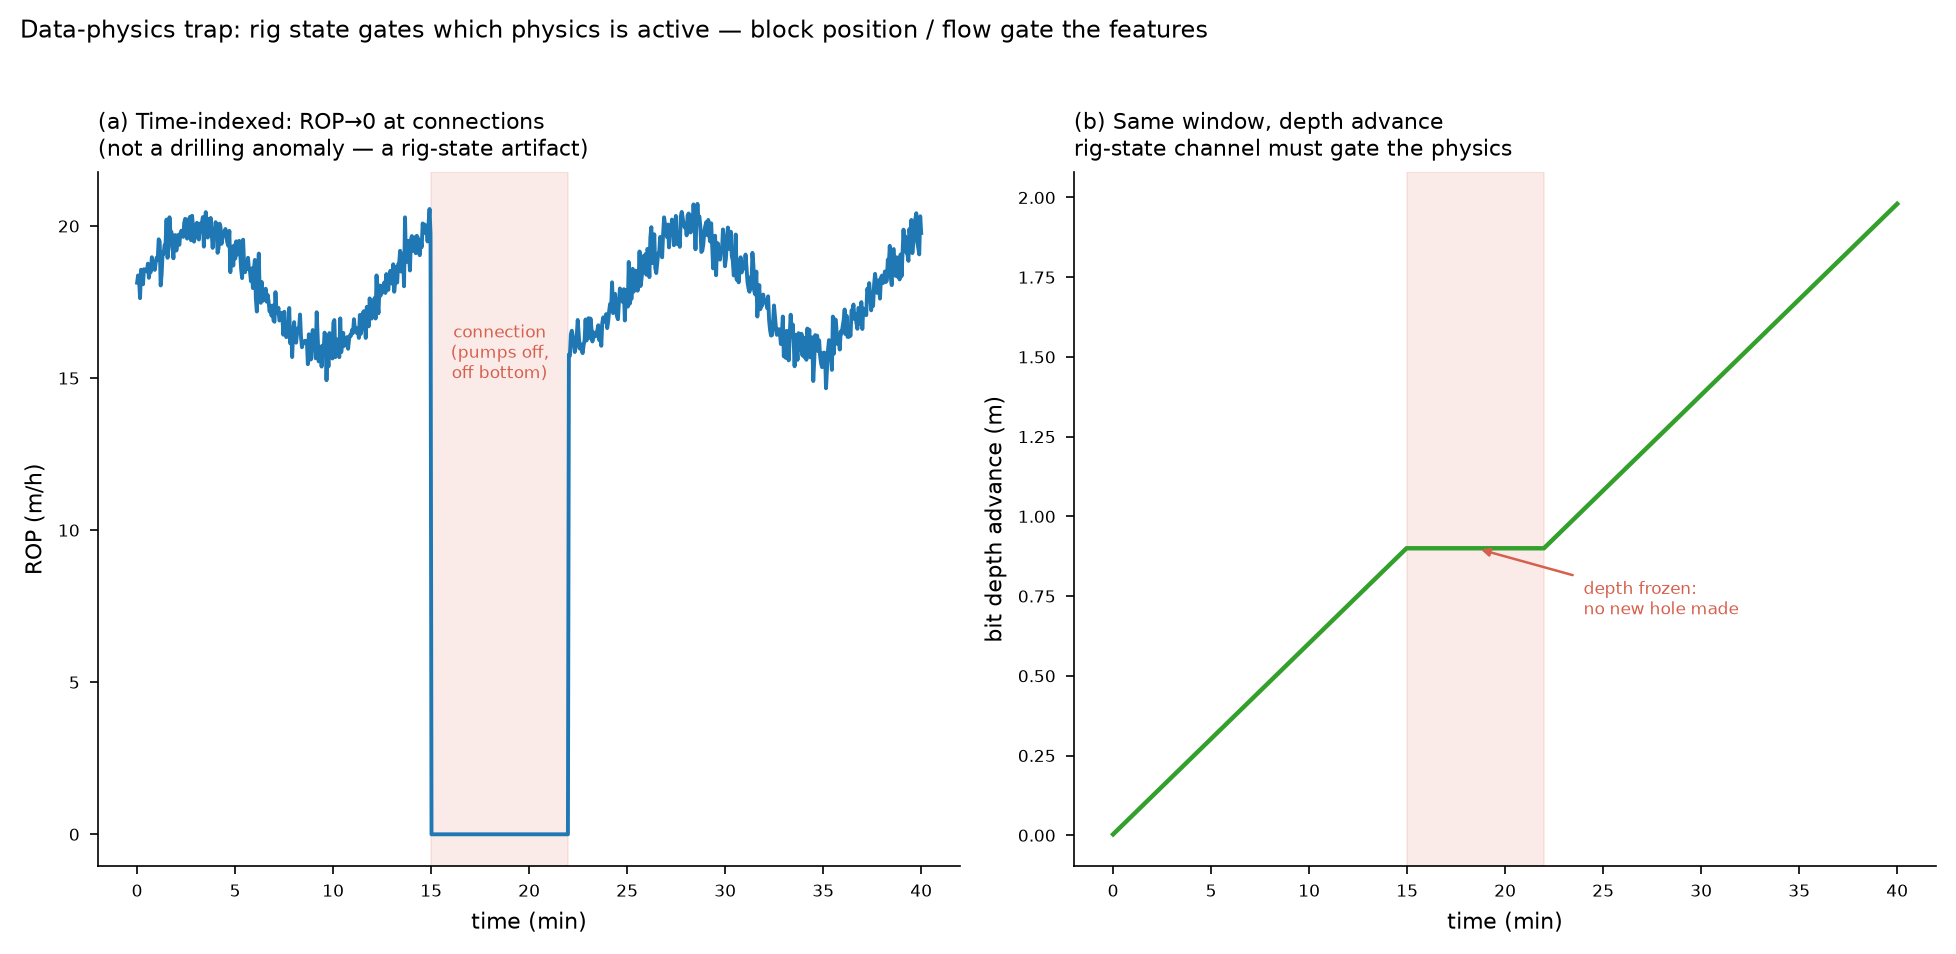
\includegraphics[width=\linewidth]{figures/fig8_timeindex_gating.png}
\caption{Why rig-state gating is required. (a) In time-indexed data the rate of penetration falls to zero at every pipe connection. (b) Bit depth is simultaneously frozen, showing the cause to be the operation rather than a developing failure. Without gating, an alarm is raised at every connection.}\label{fig:3_4}
\end{figure}

\textbf{Quality control.} Each feature carries a valid physical range. Values outside it are flagged as
\textbf{sensor faults rather than failures}, since a physically impossible reading indicates a measurement
problem. Before modelling, the computed features are checked against known physical behaviour: MSE in
efficient intervals near the expected multiple of rock strength, ECD at or above mud weight by a plausible
friction margin, and $d_c$ rising with depth under normal compaction.

\section{Model formulation and coverage-aware fusion}

Three models are applied, each matched to one of the signature classes identified in §2.11.

\textbf{Random Forest --- point classification.} An ensemble of decision trees over the per-sample feature
vector, detecting whether the current multivariate operating point resembles states labelled abnormal.
Output is a score $S_{\text{RF}} \in [0,1]$.

Labels follow a stated hierarchy, in descending preference: documented failure events with timestamps;
physics-consistency labels, requiring that *several independent features cross their thresholds together in
the correlated pattern the mechanism predicts*; and, failing both, weak heuristic labels declared as such.
The requirement of correlated multi-feature crossing is what distinguishes a physics-consistency label from
an arbitrary threshold. An anti-circularity rule applies throughout: \textbf{evaluation never reuses the rule
that generated the labels}, since a model tested against its own labelling criterion measures only its
own consistency.

\textbf{LSTM autoencoder --- temporal anomaly.} A recurrent encoder--decoder trained on \emph{normal} sequences only,
so that reconstruction error scores departure from learned dynamics. The window length is set from the
development timescale of the target mechanism rather than by convention, since a window shorter than
$\tau_{\text{dev}}$ cannot represent the precursor it is meant to detect. Output is a normalised score
$S_{\text{LSTM}} \in [0,1]$.

\textbf{Dynamic time warping --- shape matching.} Recent windows are compared against reference templates under
elastic time alignment with a Sakoe--Chiba band constraining the warping path. The \textbf{provenance of the
templates is a methodological requirement, not an implementation detail}: templates derive from the
mechanism physics of Chapter Two --- the correlated ECD, standpipe-pressure and torque ramp of a developing
pack-off; the rising-MSE, falling-ROP crossover of a dulling bit --- or from documented events. They are
never seeded from windows flagged by the autoencoder, since doing so would make the shape score a
re-encoding of the anomaly score, destroying the independence on which combining them depends. Output is
$S_{\text{DTW}} \in [0,1]$.

\textbf{Coverage-aware fusion.} The three scores combine into a single risk score, weighted and renormalised
over the monitors actually available:

\[\text{Risk}(t) = 100 \cdot \frac{\sum_{k \in \mathcal{A}(t)} w_k\,S_k(t)}{\sum_{k \in \mathcal{A}(t)} w_k}\]

where $\mathcal{A}(t)$ is the set of active monitors at time $t$ and the base weights are
$w_{\text{RF}} = 0.35$, $w_{\text{LSTM}} = 0.45$, $w_{\text{DTW}} = 0.20$.

Two properties matter. When all three monitors are active, the expression reduces exactly to the fixed
weighting --- so the fixed-weight formulation is the \emph{full-coverage special case} of the general one. When a
monitor is unavailable, the remaining weights renormalise, keeping the score on a 0--100 scale and
interpretable under reduced instrumentation rather than silently degraded.

\begin{figure}[htbp]\centering
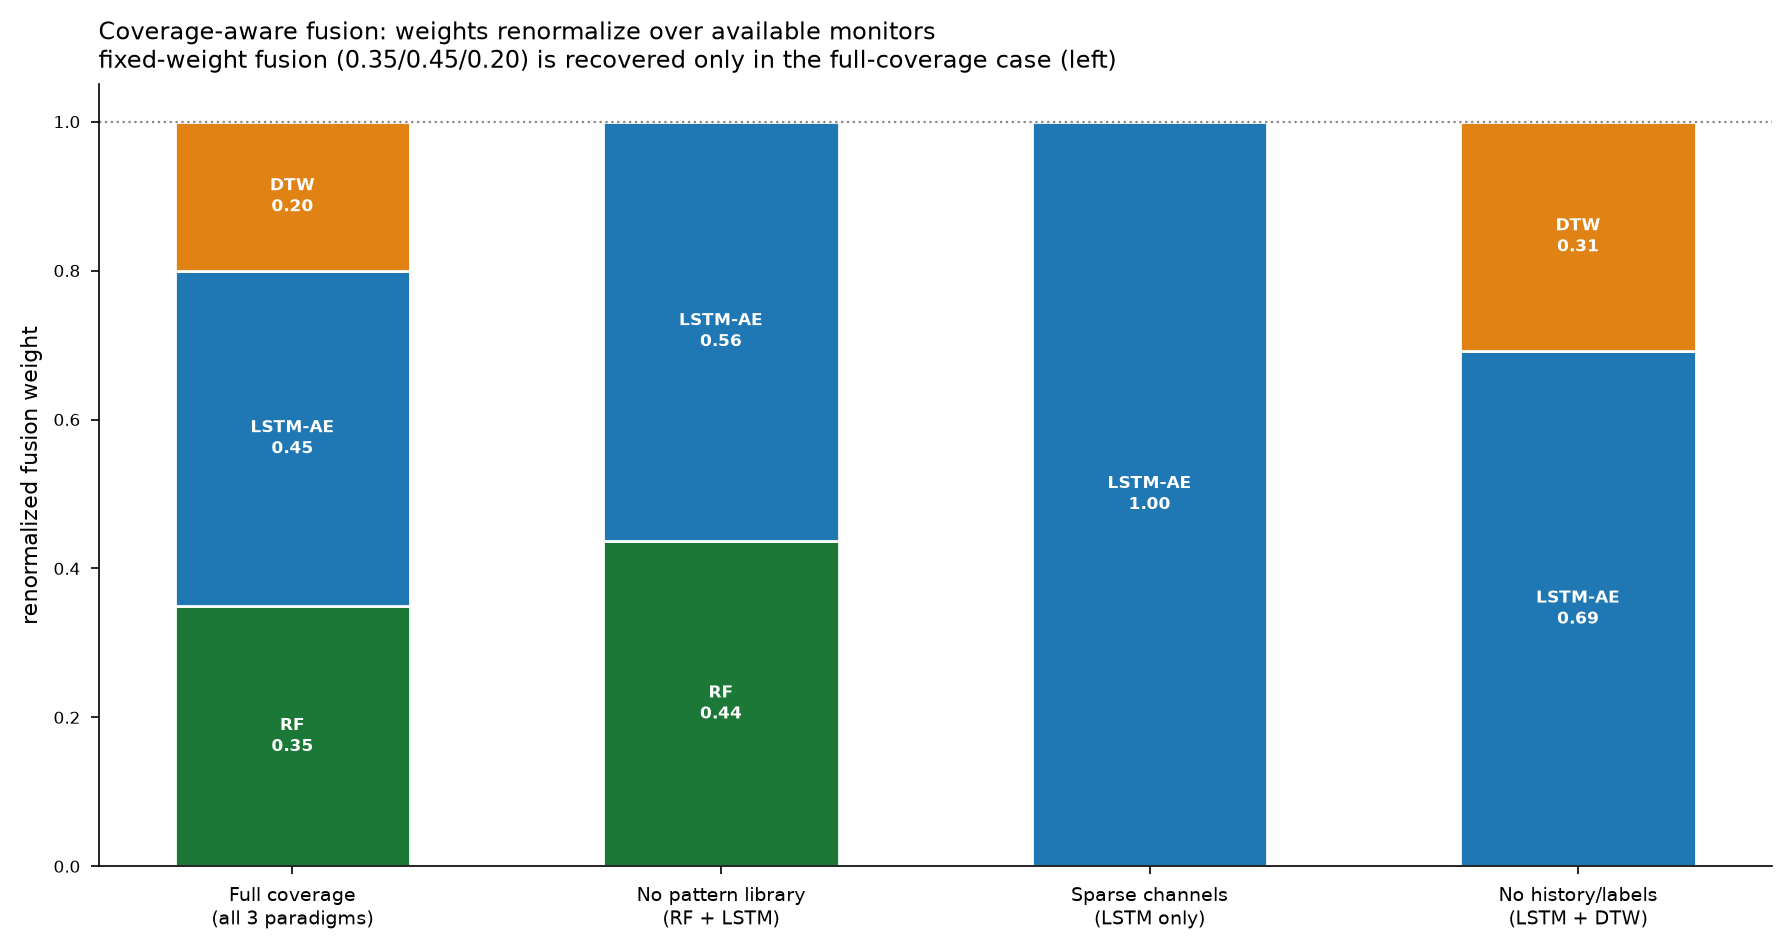
\includegraphics[width=\linewidth]{figures/fig9_coverage_fusion.png}
\caption{Coverage-aware fusion. The fixed weighting is recovered exactly under full coverage (left); as monitors become unavailable the remaining weights renormalise, so the risk score stays on a common scale under any level of instrumentation.}\label{fig:3_5}
\end{figure}

The weighting itself is a physical statement rather than a tuned constant. The heaviest weight rests on the
sequence model because the mechanisms with the longest lead times --- pack-off and bit wear --- develop as
gradual correlated trends, which is precisely what reconstruction error over a sequence detects. Point
classification and shape matching carry lower weights because their signature classes are, for these
mechanisms, secondary.

\textbf{Alert tiers and coverage reporting.} The risk score maps to four tiers spanning normal operation,
watch, elevated and action. Every score is reported together with the monitors that were active and the
mechanisms that were unobservable given the available channels --- so a risk value is never presented
without the coverage that produced it.

\section{Evaluation design}

\textbf{Anchoring.} Latency and lead time are measured relative to an anchor. Where documented timestamped
failure events exist for the well analysed, they serve as anchors and the evaluation is a labelled
validation. Where they do not, anchors are the onsets of physics-derived signatures from Chapter Two, and
the evaluation is a demonstration of physically-consistent behaviour. Which of the two applies is stated
explicitly rather than left implicit.

\textbf{Metrics.} Detection latency is the interval from anchor onset to the first alert at or above the tier
threshold; a negative latency is a lead time. Detection rate is the fraction of anchors detected within a
stated horizon, and false-alarm rate the number of alerts in windows containing no anchor, per unit
drilling time. The alert threshold is held constant across compared configurations, and results are
reported over a sweep of thresholds so that no conclusion rests on a single arbitrary cut.

\textbf{Ablation design.} The central claims are comparative, so three arms are evaluated.

\emph{Arm A --- parameter coupling:} a single channel, then two, then the full minimum observable set, then all
available channels. This isolates the contribution of coupling between parameters.

\emph{Arm B --- model fusion:} each model alone, then the fused score. This isolates the contribution of
combining signature classes.

\emph{Arm C --- composability and graceful degradation:} several representative channel subsets, for each of which
the system must derive the observable mechanisms, declare the unobservable ones, and renormalise the fusion
weights. The contrast between a self-diagnostic single channel and a relational single channel is the
sharpest test of the coupling claim of §2.10: the physics predicts the former performs acceptably alone and
the latter does not.

\textbf{Validation against physics predictions.} Because Chapter Two makes advance predictions, the results are
tested against them: no leading channel should be found for differential sticking, mechanical sticking or
kicks, and the leading channels for pack-off should be ECD, standpipe pressure and torque specifically. A
disagreement is reported as a finding rather than reconciled, since a genuine precursor where none is
predicted would be a correction to the physics.

\textbf{Guarding against leakage.} Training and test partitions are formed by well or by contiguous time block,
never by random sampling of individual samples: at intervals of seconds, adjacent samples are near
duplicates, and random partitioning would place near-identical records on both sides of the split and
inflate every metric.

\section*{References}

Sakoe, H. \& Chiba, S. (1978) \emph{Dynamic programming algorithm optimization for spoken word recognition.}
IEEE Transactions on Acoustics, Speech and Signal Processing. DOI: 10.1109/tassp.1978.1163055

Teale, R. (1965) \emph{The concept of specific energy in rock drilling.} International Journal of Rock
Mechanics and Mining Sciences. DOI: 10.1016/0148-9062(65)90022-7

*(Full reference list as given in Chapter Two; sources for the governing relations implemented in §3.2 are
cited there.)*


\end{document}
